%%%%%%%%%%%%%%%%%%%%%%%%%%%%%%%%%%%%%%%%%%%%%%%%%%%%%%%%%%%%%%%%%%%%%%
% Template for a UBC-compliant dissertation
% At the minimum, you will need to change the information found
% after the "Document meta-data"
%
%!TEX TS-program = pdflatex
%!TEX encoding = UTF-8 Unicode

%% The ubcdiss class provides several options:
%%   gpscopy (aka fogscopy)
%%       set parameters to exactly how GPS specifies
%%         * single-sided
%%         * page-numbering starts from title page
%%         * the lists of figures and tables have each entry prefixed
%%           with 'Figure' or 'Table'
%%       This can be tested by `\ifgpscopy ... \else ... \fi'
%%   10pt, 11pt, 12pt
%%       set default font size
%%   oneside, twoside
%%       whether to format for single-sided or double-sided printing
%%   balanced
%%       when double-sided, ensure page content is centred
%%       rather than slightly offset (the default)
%%   singlespacing, onehalfspacing, doublespacing
%%       set default inter-line text spacing; the ubcdiss class
%%       provides \textspacing to revert to this configured spacing
%%   draft
%%       disable more intensive processing, such as including
%%       graphics, etc.
%%

% For submission to GPS
\documentclass[gpscopy,onehalfspacing,11pt]{ubcdiss}

% change margins
\usepackage[margin=1.25in ,top=1.25in ,bottom=1.25in]{geometry}

% For your own copies (looks nicer)
% \documentclass[balanced,twoside,11pt]{ubcdiss}

%%%%%%%%%%%%%%%%%%%%%%%%%%%%%%%%%%%%%%%%%%%%%%%%%%%%%%%%%%%%%%%%%%%%%%
%%%%%%%%%%%%%%%%%%%%%%%%%%%%%%%%%%%%%%%%%%%%%%%%%%%%%%%%%%%%%%%%%%%%%%
%%
%% FONTS:
%%
%% The defaults below configures Times Roman for the serif font,
%% Helvetica for the sans serif font, and Courier for the
%% typewriter-style font.  Configuring fonts can be time
%% consuming; we recommend skipping to END FONTS!
%%
%% If you're feeling brave, have lots of time, and wish to use one
%% your platform's native fonts, see the commented out bits below for
%% XeTeX/XeLaTeX.  This is not for the faint at heart.
%% (And shouldn't you be writing? :-)
%%

%% NFSS font specification (New Font Selection Scheme)
\usepackage{times,mathptmx,courier}
\usepackage[scaled=.92]{helvet}

%% Math or theory people may want to include the handy AMS macros
%\usepackage{amssymb}
%\usepackage{amsmath}
%\usepackage{amsfonts}

%% The pifont package provides access to the elements in the dingbat font.
%% Use \ding{##} for a particular dingbat (see p7 of psnfss2e.pdf)
%%   Useful:
%%     51,52 different forms of a checkmark
%%     54,55,56 different forms of a cross (saltyre)
%%     172-181 are 1-10 in open circle (serif)
%%     182-191 are 1-10 black circle (serif)
%%     192-201 are 1-10 in open circle (sans serif)
%%     202-211 are 1-10 in black circle (sans serif)
%% \begin{dinglist}{##}\item... or dingautolist (which auto-increments)
%% to create a bullet list with the provided character.
\usepackage{pifont}

%%%%%%%%%%%%%%%%%%%%%%%%%%%%%%%%%%%%%%%%%%%%%%%%%%%%%%%%%%%%%%%%%%%%%%
%% Configure fonts for XeTeX / XeLaTeX using the fontspec package.
%% Be sure to check out the fontspec documentation.
%\usepackage{fontspec,xltxtra,xunicode}	% required
%\defaultfontfeatures{Mapping=tex-text}	% recommended
%% Minion Pro and Myriad Pro are shipped with some versions of
%% Adobe Reader.  Adobe representatives have commented that these
%% fonts can be used outside of Adobe Reader.
%\setromanfont[Numbers=OldStyle]{Minion Pro}
%\setsansfont[Numbers=OldStyle,Scale=MatchLowercase]{Myriad Pro}
%\setmonofont[Scale=MatchLowercase]{Andale Mono}

%% Other alternatives:
%\setromanfont[Mapping=tex-text]{Adobe Caslon}
%\setsansfont[Scale=MatchLowercase]{Gill Sans}
%\setsansfont[Scale=MatchLowercase,Mapping=tex-text]{Futura}
%\setmonofont[Scale=MatchLowercase]{Andale Mono}
%\newfontfamily{\SYM}[Scale=0.9]{Zapf Dingbats}
%% END FONTS
%%%%%%%%%%%%%%%%%%%%%%%%%%%%%%%%%%%%%%%%%%%%%%%%%%%%%%%%%%%%%%%%%%%%%%
%%%%%%%%%%%%%%%%%%%%%%%%%%%%%%%%%%%%%%%%%%%%%%%%%%%%%%%%%%%%%%%%%%%%%%



%%%%%%%%%%%%%%%%%%%%%%%%%%%%%%%%%%%%%%%%%%%%%%%%%%%%%%%%%%%%%%%%%%%%%%
%%%%%%%%%%%%%%%%%%%%%%%%%%%%%%%%%%%%%%%%%%%%%%%%%%%%%%%%%%%%%%%%%%%%%%
%%
%% Recommended packages
%%
\usepackage{checkend}	% better error messages on left-open environments
\usepackage{graphicx}	% for incorporating external images

%% booktabs: provides some special commands for typesetting tables as used
%% in excellent journals.  Ignore the examples in the Lamport book!
\usepackage{booktabs}

%% listings: useful support for including source code listings, with
%% optional special keyword formatting.  The \lstset{} causes
%% the text to be typeset in a smaller sans serif font, with
%% proportional spacing.
\usepackage{listings}
\lstset{basicstyle=\sffamily\scriptsize,showstringspaces=false,fontadjust}

%% The acronym package provides support for defining acronyms, providing
%% their expansion when first used, and building glossaries.  See the
%% example in glossary.tex and the example usage throughout the example
%% document.
%% NOTE: to use \MakeTextLowercase in the \acsfont command below,
%%   we *must* use the `nohyperlinks' option -- it causes errors with
%%   hyperref otherwise.  See Section 5.2 in the ``LaTeX 2e for Class
%%   and Package Writers Guide'' (clsguide.pdf) for details.
\usepackage[printonlyused,nohyperlinks]{acronym}
%% The ubcdiss.cls loads the `textcase' package which provides commands
%% for upper-casing and lower-casing text.  The following causes
%% the acronym package to typeset acronyms in small-caps
%% as recommended by Bringhurst.
\renewcommand{\acsfont}[1]{{\scshape \MakeTextLowercase{#1}}}

%% color: add support for expressing colour models.  Grey can be used
%% to great effect to emphasize other parts of a graphic or text.
%% For an excellent set of examples, see Tufte's "Visual Display of
%% Quantitative Information" or "Envisioning Information".
\usepackage{color}
\definecolor{greytext}{gray}{0.5}

%% comment: provides a new {comment} environment: all text inside the
%% environment is ignored.
%%   \begin{comment} ignored text ... \end{comment}
\usepackage{comment}

%% The natbib package provides more sophisticated citing commands
%% such as \citeauthor{} to provide the author names of a work,
%% \citet{} to produce an author-and-reference citation,
%% \citep{} to produce a parenthetical citation.
%% We use \citeeg{} to provide examples
\usepackage[numbers,sort&compress]{natbib}
\newcommand{\citeeg}[1]{\citep[e.g.,][]{#1}}

%% The titlesec package provides commands to vary how chapter and
%% section titles are typeset.  The following uses more compact
%% spacings above and below the title.  The titleformat that follow
%% ensure chapter/section titles are set in singlespace.
\usepackage[compact]{titlesec}
\titleformat*{\section}{\singlespacing\raggedright\bfseries\Large}
\titleformat*{\subsection}{\singlespacing\raggedright\bfseries\large}
\titleformat*{\subsubsection}{\singlespacing\raggedright\bfseries}
\titleformat*{\paragraph}{\singlespacing\raggedright\itshape}

%% The caption package provides support for varying how table and
%% figure captions are typeset.
\usepackage[format=hang,indention=-1cm,labelfont={bf},margin=1em]{caption}

%% url: for typesetting URLs and smart(er) hyphenation.
%% \url{http://...}
\usepackage{url}
\urlstyle{sf}	% typeset urls in sans-serif


%%%%%%%%%%%%%%%%%%%%%%%%%%%%%%%%%%%%%%%%%%%%%%%%%%%%%%%%%%%%%%%%%%%%%%
%%%%%%%%%%%%%%%%%%%%%%%%%%%%%%%%%%%%%%%%%%%%%%%%%%%%%%%%%%%%%%%%%%%%%%
%%
%% Possibly useful packages: you may need to explicitly install
%% these from CTAN if they aren't part of your distribution;
%% teTeX seems to ship with a smaller base than MikTeX and MacTeX.
%%
%\usepackage{pdfpages}	% insert pages from other PDF files
\usepackage{longtable}	% provide tables spanning multiple pages
%\usepackage{chngpage}	% support changing the page widths on demand
%\usepackage{tabularx}	% an enhanced tabular environment
\usepackage{pdflscape} % to make landscape pages

\usepackage{array} % for changing alignment within cells in longtable

%% enumitem: support pausing and resuming enumerate environments.
%\usepackage{enumitem}

%% rotating: provides two environments, sidewaystable and sidewaysfigure,
%% for typesetting tables and figures in landscape mode.
%\usepackage{rotating}

%% subfig: provides for including subfigures within a figure,
%% and includes being able to separately reference the subfigures.
%\usepackage{subfig}

%% ragged2e: provides several new new commands \Centering, \RaggedLeft,
%% \RaggedRight and \justifying and new environments Center, FlushLeft,
%% FlushRight and justify, which set ragged text and are easily
%% configurable to allow hyphenation.
%\usepackage{ragged2e}

%% The ulem package provides a \sout{} for striking out text and
%% \xout for crossing out text.  The normalem and normalbf are
%% necessary as the package messes with the emphasis and bold fonts
%% otherwise.
%\usepackage[normalem,normalbf]{ulem}    % for \sout

%%%%%%%%%%%%%%%%%%%%%%%%%%%%%%%%%%%%%%%%%%%%%%%%%%%%%%%%%%%%%%%%%%%%%%
%% HYPERREF:
%% The hyperref package provides for embedding hyperlinks into your
%% document.  By default the table of contents, references, citations,
%% and footnotes are hyperlinked.
%%
%% Hyperref provides a very handy command for doing cross-references:
%% \autoref{}.  This is similar to \ref{} and \pageref{} except that
%% it automagically puts in the *type* of reference.  For example,
%% referencing a figure's label will put the text `Figure 3.4'.
%% And the text will be hyperlinked to the appropriate place in the
%% document.
%%
%% Generally hyperref should appear after most other packages

%% The following puts hyperlinks in very faint grey boxes.
%% The `pagebackref' causes the references in the bibliography to have
%% back-references to the citing page; `backref' puts the citing section
%% number.  See further below for other examples of using hyperref.
%% 2009/12/09: now use `linktocpage' (Jacek Kisynski): GPS now prefers
%%   that the ToC, LoF, LoT place the hyperlink on the page number,
%%   rather than the entry text.
\usepackage[bookmarks,bookmarksnumbered,%
    allbordercolors={0.8 0.8 0.8},%
    pagebackref,linktocpage%
    ]{hyperref}
%% The following change how the the back-references text is typeset in a
%% bibliography when `backref' or `pagebackref' are used
\renewcommand\backrefpagesname{\(\rightarrow\) pages}
\renewcommand\backref{\textcolor{greytext} \backrefpagesname\ }

%% The following uses most defaults, which causes hyperlinks to be
%% surrounded by colourful boxes; the colours are only visible in
%% PDFs and don't show up when printed:
%\usepackage[bookmarks,bookmarksnumbered]{hyperref}

%% The following disables the colourful boxes around hyperlinks.
%\usepackage[bookmarks,bookmarksnumbered,pdfborder={0 0 0}]{hyperref}

%% The following disables all hyperlinking, but still enabled use of
%% \autoref{}
%\usepackage[draft]{hyperref}

%% The following commands causes chapter and section references to
%% uppercase the part name.
\renewcommand{\chapterautorefname}{Chapter}
\renewcommand{\sectionautorefname}{Section}
\renewcommand{\subsectionautorefname}{Section}
\renewcommand{\subsubsectionautorefname}{Section}

%% If you have long page numbers (e.g., roman numbers in the
%% preliminary pages for page 28 = xxviii), you might need to
%% uncomment the following and tweak the \@pnumwidth length
%% (default: 1.55em).  See the tocloft documentation at
%% http://www.ctan.org/tex-archive/macros/latex/contrib/tocloft/
% \makeatletter
% \renewcommand{\@pnumwidth}{3em}
% \makeatother

%%%%%%%%%%%%%%%%%%%%%%%%%%%%%%%%%%%%%%%%%%%%%%%%%%%%%%%%%%%%%%%%%%%%%%
%%%%%%%%%%%%%%%%%%%%%%%%%%%%%%%%%%%%%%%%%%%%%%%%%%%%%%%%%%%%%%%%%%%%%%
%%
%% Some special settings that controls how text is typeset
%%
% \raggedbottom		% pages don't have to line up nicely on the last line
% \sloppy		% be a bit more relaxed in inter-word spacing
% \clubpenalty=10000	% try harder to avoid orphans
% \widowpenalty=10000	% try harder to avoid widows
% \tolerance=1000

%% And include some of our own useful macros
% This file provides examples of some useful macros for typesetting
% dissertations.  None of the macros defined here are necessary beyond
% for the template documentation, so feel free to change, remove, and add
% your own definitions.
%
% We recommend that you define macros to separate the semantics
% of the things you write from how they are presented.  For example,
% you'll see definitions below for a macro \file{}: by using
% \file{} consistently in the text, we can change how filenames
% are typeset simply by changing the definition of \file{} in
% this file.
% 
%% The following is a directive for TeXShop to indicate the main file
%%!TEX root = diss.tex

\newcommand{\NA}{\textsc{n/a}}	% for "not applicable"
\newcommand{\eg}{e.g.,\ }	% proper form of examples (\eg a, b, c)
\newcommand{\ie}{i.e.,\ }	% proper form for that is (\ie a, b, c)
\newcommand{\etal}{\emph{et al}}

% Some useful macros for typesetting terms.
\newcommand{\file}[1]{\texttt{#1}}
\newcommand{\class}[1]{\texttt{#1}}
\newcommand{\latexpackage}[1]{\href{http://www.ctan.org/macros/latex/contrib/#1}{\texttt{#1}}}
\newcommand{\latexmiscpackage}[1]{\href{http://www.ctan.org/macros/latex/contrib/misc/#1.sty}{\texttt{#1}}}
\newcommand{\env}[1]{\texttt{#1}}
\newcommand{\BibTeX}{Bib\TeX}

% Define a command \doi{} to typeset a digital object identifier (DOI).
% Note: if the following definition raise an error, then you likely
% have an ancient version of url.sty.  Either find a more recent version
% (3.1 or later work fine) and simply copy it into this directory,  or
% comment out the following two lines and uncomment the third.
\DeclareUrlCommand\DOI{}
\newcommand{\doi}[1]{\href{http://dx.doi.org/#1}{\DOI{doi:#1}}}
%\newcommand{\doi}[1]{\href{http://dx.doi.org/#1}{doi:#1}}

% Useful macro to reference an online document with a hyperlink
% as well with the URL explicitly listed in a footnote
% #1: the URL
% #2: the anchoring text
\newcommand{\webref}[2]{\href{#1}{#2}\footnote{\url{#1}}}

% epigraph is a nice environment for typesetting quotations
\makeatletter
\newenvironment{epigraph}{%
	\begin{flushright}
	\begin{minipage}{\columnwidth-0.75in}
	\begin{flushright}
	\@ifundefined{singlespacing}{}{\singlespacing}%
    }{
	\end{flushright}
	\end{minipage}
	\end{flushright}}
\makeatother

% \FIXME{} is a useful macro for noting things needing to be changed.
% The following definition will also output a warning to the console
\newcommand{\FIXME}[1]{\typeout{**FIXME** #1}\textbf{[FIXME: #1]}}

% END


%%%%%%%%%%%%%%%%%%%%%%%%%%%%%%%%%%%%%%%%%%%%%%%%%%%%%%%%%%%%%%%%%%%%%%
%%%%%%%%%%%%%%%%%%%%%%%%%%%%%%%%%%%%%%%%%%%%%%%%%%%%%%%%%%%%%%%%%%%%%%
%%
%% Document meta-data: be sure to also change the \hypersetup information
%%

\title{\scshape\bfseries Germline Pharmacogenomics Testing in Formalin-Fixed Paraffin-Embedded Tumours}
%\subtitle{If you want a subtitle}

\author{Shyong Quin Yap}
\previousdegree{B.Sc. (Hons), Trent University, 2011}

% What is this dissertation for?
\degreetitle{\scshape\bfseries Master of Science}

\institution{The University of British Columbia}
\campus{Vancouver}

\faculty{The Faculty of Graduate and Postdoctoral Studies}
\department{Experimental Medicine Program}
\submissionmonth{January}
\submissionyear{2017}

%% hyperref package provides support for embedding meta-data in .PDF
%% files
\hypersetup{
  pdftitle={Change this title!  (DRAFT: \today)},
  pdfauthor={Johnny Canuck},
  pdfkeywords={Your keywords here}
}

%%%%%%%%%%%%%%%%%%%%%%%%%%%%%%%%%%%%%%%%%%%%%%%%%%%%%%%%%%%%%%%%%%%%%%
%%%%%%%%%%%%%%%%%%%%%%%%%%%%%%%%%%%%%%%%%%%%%%%%%%%%%%%%%%%%%%%%%%%%%%
%%
%% The document content
%%

%% LaTeX's \includeonly commands causes any uses of \include{} to only
%% include files that are in the list.  This is helpful to produce
%% subsets of your thesis (e.g., for committee members who want to see
%% the dissertation chapter by chapter).  It also saves time by
%% avoiding reprocessing the entire file.
%\includeonly{intro,conclusions}
%\includeonly{discussion}

\begin{document}

%%%%%%%%%%%%%%%%%%%%%%%%%%%%%%%%%%%%%%%%%%%%%%%%%%
%% From Thesis Components: Tradtional Thesis
%% <http://www.grad.ubc.ca/current-students/dissertation-thesis-preparation/order-components>

% Preliminary Pages (numbered in lower case Roman numerals)
%    1. Title page (mandatory)
\maketitle

%    2. Abstract (mandatory - maximum 350 words)
%% The following is a directive for TeXShop to indicate the main file
%%!TEX root = diss.tex

\chapter{Abstract}

Genomic analyses of tumours can not only reveal actionable somatic mutations, but also germline variants with clinical implications for patients and their families. While sequencing of tumour-normal pairs would enable simultaneous identification of clinically important germline variants, matched normal samples are often not obtained in clinical practice. Furthermore, tumour specimens are typically formalin-fixed paraffin-embedded (FFPE), which induces DNA damage that poses challenges in molecular testing. A framework that leverages clinical tumour sequencing for germline testing is cost-saving because only patients with potential germline variants would be referred to downstream confirmatory testing. However, this would require evaluating usability of FFPE DNA for germline testing and establishing an approach to distinguish between germline and somatic variants in tumour-only analyses. We retrospectively analyzed clinical amplicon sequencing data from 213 patients with tumour and matched normal samples. To evaluate the usability of FFPE DNA for germline testing, we characterized formalin-induced DNA damage by comparing efficiency in amplicon enrichment and sequencing results of FFPE DNA to blood, the gold standard for germline testing. Although formalin-induced DNA damage including fragmentation and cytosine deamination were detectable, we determined that these discrepancies were either technically negligible or could be minimized using appropriate methods. We also found that 93.8\% of germline alterations identified in blood were present with the same allelic statuses in FFPE tumours. This implies that the majority of germline genetic changes are retained in the tumour genome, demonstrating the reliability of using tumour DNA for germline variant calling. Lastly, we assessed the application of variant allele frequency (VAF) threshold to delineate germline and somatic variants in tumour-only analyses. We reported that a VAF cut-off of 30\% would correctly identify 94\% of germline alterations, while erroneously submit 10\% of false positives, which are somatic mutations, for follow-up germline testing. This underscores the high sensitivity and precision of using VAF threshold to discriminate between germline and somatic variants in tumour-only analyses. Our results collectively demonstrate an invaluable finding in clinical genomics wherein leveraging FFPE tumour sequencing for identification of germline variants could be a practical, cost-efficient approach for providing germline testing. 

\cleardoublepage

%    3. Preface
%% The following is a directive for TeXShop to indicate the main file
%%!TEX root = diss.tex

\chapter{Preface}

This dissertation is based on next-generation sequencing data from The OncoPanel Pilot (TOP) study. The TOP study was designed to optimize and validate a clinical targeted NGS panel for its utility as standard of care. Approval of this pilot study was covered by the Human Research Ethics Protocol H14-01212. Sample preparation and sequencing, as well as processing of raw data, read alignment, and variant calling were collaboratively performed by members of Canada's Michael Smith Genome Sciences Centre and the Centre for Clinical Genomics. Data analyses in Chapter 3 and 4 are my original work.

A version of the Introduction chapter was submitted to the Ideas, Numbers, and Knowledge (INK) journal. Analysis of pharmacogenomic genes in Chapter 3 and 4 was presented as a poster titled ``Comparative Analysis of Pharmacogenomic Variants in Amplicon-sequenced DNA from Peripheral Blood and Formalin-fixed Paraffin-embedded Tumours" at the 2016 Intelligent Systems for Molecular Biology conference and the Translational Medicine (TransMed) Special Interest Group meeting.

\cleardoublepage

%    4. Table of contents (mandatory - list all items in the preliminary pages
%    starting with the abstract, followed by chapter headings and
%    subheadings, bibliographies and appendices)
\tableofcontents
\cleardoublepage	% required by tocloft package

%    5. List of tables (mandatory if thesis has tables)
\listoftables
\cleardoublepage	% required by tocloft package

%    6. List of figures (mandatory if thesis has figures)
\listoffigures
\cleardoublepage	% required by tocloft package

%    7. List of illustrations (mandatory if thesis has illustrations)
%    8. Lists of symbols, abbreviations or other (optional)

%    9. Glossary (optional)
%% The following is a directive for TeXShop to indicate the main file
%%!TEX root = diss.tex

\chapter{List of Abbreviations}

%This glossary uses the handy \latexpackage{acroynym} package to automatically
%maintain the glossary.  It uses the package's \texttt{printonlyused}
%option to include only those acronyms explicitly referenced in the
%\LaTeX\ source.

% use \acrodef to define an acronym, but no listing
% \acrodef{UI}{user interface}
% \acrodef{UBC}{University of British Columbia}

% The acronym environment will typeset only those acronyms that were
% *actually used* in the course of the document

\begin{acronym}[BCR-ABL1]
\acro{ACCE}{Analytical validity, Clinical validity, Clinical utility, and Ethical, legal and social implications}

\acro{ALK}[\textit{ALK}]{Anaplastic lymphoma kinase gene}

\acro{APC}[\textit{APC}]{Adenomatous polyposis coli gene}

\acro{BAM}{Binary Alignment$/$Map}

\acro{BAQ}{Base quality score}

\acro{BCR-ABL1}[\textit{BCR-ABL1}]{Breakpoint cluster region and Abelson murine leukemia viral oncogene homolog 1 fusion gene}

\acro{BRAF}[\textit{BRAF}]{B-Raf proto-oncogene}

\acro{BRCA1}[\textit{BRCA1}]{Breast cancer type 1 susceptibility gene}

\acro{BRCA2}[\textit{BRCA2}]{Breast cancer type 2 susceptibility gene}

\acro{BWA}{Burrows-Wheeler aligner}

\acro{BWT}{Burrows-Wheeler transform}

\acro{CDC}{Centers for Disease Control and Prevention}

\acro{COSMIC}{Catalogue of Somatic Mutations in Cancer database}

\acro{CPG}{Cancer predisposing gene}

\acro{CRC}{Colorectal cancer}

\acro{dbSNP}{Single Nucleotide Polymorphism Database}

\acro{dNTP}{Deoxyribonucleotides}

\acro{dTMP}{Deoxythymidine monophosphate}

\acro{DNA}{Deoxyribonucleic acid}

\acro{DPD}{Dihydropyrimidine dehydrogenase enzyme}

\acro{DPYD}[\textit{DPYD}]{Dihydropyrimidine dehydrogenase gene}

\acro{EGFR}[\textit{EGFR}]{Epidermal growth factor receptor gene}

\acro{ExAC}{Exome Aggregation Consortium}

\acro{FAP}{Familial adenomatous polyposis}

\acro{FET}{Fisher's exact test}

\acro{FFPE}{Formalin-fixed Paraffin-embedded}

\acro{GIST}{Gastrointestinal stromal tumour}

\acro{GSH}{Glutathione}

\acro{GSTP}{Glutathione S-transferases}

\acro{GSTP1}[\textit{GSTP1}]{Glutathione S-transferases gene}

\acro{HER2}[\textit{HER2}]{Human epidermal growth factor receptor 2 gene}

\acro{HGP}{Human Genome Project}

\acro{ICGC}{International Cancer Genome Consortium}

\acro{IGV}{Intergrative Genomics Viewer}

\acro{LOH}{Loss of heterozygosity}

\acro{MAPQ}{Mapping quality score}

\acro{MIT}{Massachusetts Institute of Technology}

\acro{MEN2}{Multiple endocrine neoplasia type 2}

\acro{MR}{Methylenetetrahydrofolate reductase enzyme}

\acro{MTHFR}[\textit{MTHFR}]{Methylenetetrahydrofolate reductase gene}

\acro{NHGRI}{National Human Genome Research Institute}

\acro{NGS}{Next-generation sequencing}

\acro{PGx}{Pharmacogenomics}

\acro{PCR}{Polymerase chain reaction}

\acro{PPV}{Positive predictive value}

\acro{RB1}[\textit{RB1}]{Retinoblastoma 1 gene}

\acro{RET}[\textit{RET}]{Ret proto-oncogene}

\acro{SAM}{Sequence Alignment$/$Map}

\acro{TCGA}{The Cancer Genome Atlas}

\acro{TP53}[\textit{TP53}]{Tumour protein p53 gene}

\acro{TP}{Thymidine phosphorylase enzyme}

\acro{TS}{Thymidylate synthase enzyme}

\acro{TYMP}[\textit{TYMP}]{Thymidine phosphorylase gene}

\acro{TYMS}[\textit{TYMS}]{Thymidylate synthase gene}

\acro{UDG}{Rracil-DNA glycosylase}

\acro{UGT1A}{Uridine diphosphate glycosyltransferase 1 family enzymes}

\acro{UGT1A1}[\textit{UGT1A1}]{Uridine diphosphate glycosyltransferase 1A1 gene}

\acro{VAF}{Variant allele frequency}

\acro{VCF}{Variant Call Format}

\acro{WES}{Whole exome sequencing}

\acro{WGS}{Whole genome sequencing}

\acro{ANOVA}[ANOVA]{Analysis of Variance\acroextra{, a set of
  statistical techniques to identify sources of variability between groups}}
\acro{API}{application programming interface}
\acro{CTAN}{\acroextra{The }Common \TeX\ Archive Network}
\acro{DOI}{Document Object Identifier\acroextra{ (see
    \url{http://doi.org})}}
\acro{GPS}[GPS]{Graduate and Postdoctoral Studies}
\acro{PDF}{Portable Document Format}
\acro{RCS}[RCS]{Revision control system\acroextra{, a software
    tool for tracking changes to a set of files}}
\acro{TLX}[TLX]{Task Load Index\acroextra{, an instrument for gauging
  the subjective mental workload experienced by a human in performing
  a task}}
\acro{UML}{Unified Modelling Language\acroextra{, a visual language
    for modelling the structure of software artefacts}}
\acro{URL}{Unique Resource Locator\acroextra{, used to describe a
    means for obtaining some resource on the world wide web}}
\acro{W3C}[W3C]{\acroextra{the }World Wide Web Consortium\acroextra{,
    the standards body for web technologies}}
\acro{XML}{Extensible Markup Language}
\acro{VUS}{Variant of Unknown Significance}
\end{acronym}

% You can also use \newacro{}{} to only define acronyms
% but without explictly creating a glossary
%
% \newacro{ANOVA}[ANOVA]{Analysis of Variance\acroextra{, a set of
%   statistical techniques to identify sources of variability between groups.}}
% \newacro{API}[API]{application programming interface}
% \newacro{GOMS}[GOMS]{Goals, Operators, Methods, and Selection\acroextra{,
%   a framework for usability analysis.}}
% \newacro{TLX}[TLX]{Task Load Index\acroextra{, an instrument for gauging
%   the subjective mental workload experienced by a human in performing
%   a task.}}
% \newacro{UI}[UI]{user interface}
% \newacro{UML}[UML]{Unified Modelling Language}
% \newacro{W3C}[W3C]{World Wide Web Consortium}
% \newacro{XML}[XML]{Extensible Markup Language}

\endinput
	% always input, since other macros may rely on it

\textspacing		% begin one-half or double spacing

%   10. Acknowledgements (optional)
%% The following is a directive for TeXShop to indicate the main file
%%!TEX root = diss.tex

\chapter{Acknowledgments}

I would like to thank my supervisor, Dr. Aly Karsan for giving me the opportunity to undertake a bioinformatics project for my Master's thesis and funding me throughout the course of my research. My gratitude is extended to my committee members, Dr. Martin Hirst and Dr. Ryan Morin for providing guidance and ideas in data analyses for my project. I am also grateful for the productive discussions I had with members from the Center for Clinical Genomics and Karsan lab.

There were many individuals who endured my frustration yet provided me with endless support and encouragement. For that, I would like to express my heartfelt gratitude to my family, my academic mentor, Dr. David Walker, and my friends. Thank you James Topham, Jenny Zhao, Jessica Pilsworth, Joey Ip, Kate Slowski, Ka Ming Nip, Laura Graziano, Patrick Coulombe, Samiah Alam, Samantha Jones, Santina Lin, Tehmina Masud, and Yuko Goto for keeping me motivated and sane throughout this journey. Last but not least, I would like to thank my partner, Florian Krauthan for comforting me in my moments of failures, celebrating my successes, and understanding why dirty dishes were left in the sink.


%   11. Dedication (optional)

% Body of Thesis (not all sections may apply)
\mainmatter

\acresetall	% reset all acronyms used so far

%    1. Introduction
%% The following is a directive for TeXShop to indicate the main file
%%!TEX root = diss.tex

\chapter{Introduction}
\label{ch:Introduction}

This chapter will introduce causative factors

%%%%%%%%%%%%%%%%%%%%%%%%%%%%%%%%%%%%%%%%%%%%%%%%%%%%%%%%%%%%%%%%%%%%%%
\section{Cancer as an (Epi)genetic Disease}
\label{sec:Cancerasan(Epi)geneticDisease}

Cancer is a group of disorders defined by abnormal cell growth. Although fundamentally known to arise from genetic mutations, the disease paradigm has expanded to include aberrant epigenetic mechanisms as a contributing factor to oncogenesis.
The understanding of cancer pathogenesis has expanded been increasing over the years and a disorder that was fundamentally known to arise from genetic mutations this group of disorders which have been fundamentally known Cancer has been fundamentally known as a genetic disease defined by abnormal proliferation of cells.
Our understanding of cancer pathogenesis has been expanding  Although the understanding of cancer pathogenesis has been expanding, Cancer has been fundamentally known as a genetic disease.

Intro Outline
- Causative roles of genetic and epigenetic changes in cancers

What led to development of precision medicine?
- Precision oncology revolutionized by NGS types and technologies and bioinformatics pipelines
- Pros and cons of NGS types: Targeted, whole exome, RNA sequencing, and whole genome sequencing
- NGS technologies: how it is mostly Illumina
- Bioinformatics pipelines: alignment, variant calling algorithms, manual review

What is promising about precision medicine?
- Administration of targeted therapies and therapeutic interventions guided by cancer pharmacogenomics

- Challenges in precision medicine: formalin artifacts, tumour-only profiling, cost, turn-around time, accurate reference genome

%%%%%%%%%%%%%%%%%%%%%%%%%%%%%%%%%%%%%%%%%%%%%%%%%%%%%%%%%%%%%%%%%%%%%%
\section{The Era of Precision Oncology}
\label{sec:TheEraofPrecisionOncology}

The era of precision oncology has been revolutionized by NGS technologies and bioinformatics algorithms etc. This results in the use of molecular targeted therapies to treat patients and PGx info to administer chemo.

\subsection{Next-Generation Sequencing Technologies in the Clinic}

\subsection{Clinical Application of Bioinformatics Pipelines}

\subsection{Molecular Targeted Therapies}

\subsection{Cancer Pharmacogenomics}

%%%%%%%%%%%%%%%%%%%%%%%%%%%%%%%%%%%%%%%%%%%%%%%%%%%%%%%%%%%%%%%%%%%%%%
\section{Challenges in Clinical Applications of Next-Generation Sequencing}
\label{sec:ChallengesinClinicalApplicationsofNext-GenerationSequencing}

\subsection{Formalin-Fixed Clinical Specimens}

\subsection{Tumour-Only Profiling}

%%%%%%%%%%%%%%%%%%%%%%%%%%%%%%%%%%%%%%%%%%%%%%%%%%%%%%%%%%%%%%%%%%%%%%
\section{BibTeX}
\label{sec:BibTeX}

One of the primary benefits of using \LaTeX\ is its companion program,
\BibTeX, for managing bibliographies and citations.  Managing
bibliographies has three parts: (i) describing references,
(ii)~citing references, and (iii)~formatting cited references.

\subsection{Describing References}

\BibTeX\ defines a standard format for recording details about a
reference.  These references are recorded in a file with a
\file{.bib} extension.  \BibTeX\ supports a broad range of
references, such as books, articles, items in a conference proceedings,
chapters, technical reports, manuals, dissertations, and unpublished
manuscripts.
A reference may include attributes such as the authors,
the title, the page numbers, the \ac{DOI}, or a \ac{URL}.  A reference
can also be augmented with personal attributes, such as a rating,
notes, or keywords.

Each reference must be described by a unique \emph{key}.\footnote{%
    Note that the citation keys are different from the reference
    identifiers as described in \autoref{sec:CrossReferences}.}
A key is a simple sequence of characters, numbers, digits, and some
punctuation marks such as ``:'' and ``--''; there should be no spaces.
A consistent key format simiplifies remembering how to make references.
For example:
\begin{quote}
   \fbox{\emph{last-name}}\texttt{-}\fbox{\emph{year}}\texttt{-}\fbox{\emph{contracted-title}}
\end{quote}
where \emph{last-name} represents the last name for the first author,
and \emph{contracted-title} is some meaningful contraction of the
title.  Then \citeauthor{kiczales-1997-aop}'s seminal article on
aspect-oriented programming~\cite{kiczales-1997-aop} (published in
\citeyear{kiczales-1997-aop}) might be given the key
\texttt{kiczales-1997-aop}.

An example of a \BibTeX\ \file{.bib} file is included as
\file{biblio.bib}.  A description of the format a \file{.bib}
file is beyond the scope of this document.  We instead encourage
you to use one of the several reference managers that support the
\BibTeX\ format such as
\webref{http://jabref.sourceforge.net}{JabRef} (multiple platforms) or
\webref{http://bibdesk.sourceforge.net}{BibDesk} (MacOS\,X only).
These front ends are similar to reference manages such as
EndNote or RefWorks.


\subsection{Citing References}

Having described some references, we then need to cite them.  We
do this using a form of the \verb+\cite+ command.  For example:
\begin{lstlisting}
    \citet{kiczales-1997-aop} present examples of crosscutting
    from programs written in several languages.
\end{lstlisting}
When processed, the \verb+\citet+ will cause the paper's authors
and a standardized reference to the paper to be inserted in the
document, and will also include a formatted citation for the paper
in the bibliography.  For example:
\begin{quote}
    \citet{kiczales-1997-aop} present examples of crosscutting
    from programs written in several languages.
\end{quote}
There are several forms of the \verb+\cite+ command (provided
by the \latexpackage{natbib} package), as demonstrated in
\autoref{tbl:natbib:cite}.
Note that the form of the citation (numeric or author-year) depends
on the bibliography style (described in the next section).
The \verb+\citet+ variant is used when the author names form
an object in the sentence, whereas the \verb+\citep+ variant
is used for parenthetic references, more like an end-note.
\begin{table}
\caption{Available \texttt{cite} variants; the exact citation style
    depends on whether the bibliography style is numeric or author-year.}
\label{tbl:natbib:cite}
\centering
\begin{tabular}{lp{3.25in}}\toprule
Variant & Result \\
\midrule
% We cheat here to simulate the cite/citep/citet for APA-like styles
\verb+\cite+ & Parenthetical citation (\eg ``\cite{kiczales-1997-aop}''
    or ``(\citeauthor{kiczales-1997-aop} \citeyear{kiczales-1997-aop})'') \\
\verb+\citet+ & Textual citation: includes author (\eg
    ``\citet{kiczales-1997-aop}'' or
    or ``\citeauthor{kiczales-1997-aop} (\citeyear{kiczales-1997-aop})'') \\
\verb+\citet*+ & Textual citation with unabbreviated author list \\
\verb+\citealt+ & Like \verb+\citet+ but without parentheses \\
\verb+\citep+ & Parenthetical citation (\eg ``\cite{kiczales-1997-aop}''
    or ``(\citeauthor{kiczales-1997-aop} \citeyear{kiczales-1997-aop})'') \\
\verb+\citep*+ & Parenthetical citation with unabbreviated author list \\
\verb+\citealp+ & Like \verb+\citep+ but without parentheses \\
\verb+\citeauthor+ & Author only (\eg ``\citeauthor{kiczales-1997-aop}'') \\
\verb+\citeauthor*+ & Unabbreviated authors list
    (\eg ``\citeauthor*{kiczales-1997-aop}'') \\
\verb+\citeyear+ & Year of citation (\eg ``\citeyear{kiczales-1997-aop}'') \\
\bottomrule
\end{tabular}
\end{table}

\subsection{Formatting Cited References}

\BibTeX\ separates the citing of a reference from how the cited
reference is formatted for a bibliography, specified with the
\verb+\bibliographystyle+ command.
There are many varieties, such as \texttt{plainnat}, \texttt{abbrvnat},
\texttt{unsrtnat}, and \texttt{vancouver}.
This document was formatted with \texttt{abbrvnat}.
Look through your \TeX\ distribution for \file{.bst} files.
Note that use of some \file{.bst} files do not emit all the information
necessary to properly use \verb+\citet{}+, \verb+\citep{}+,
\verb+\citeyear{}+, and \verb+\citeauthor{}+.

There are also packages available to place citations on a per-chapter
basis (\latexpackage{bibunits}), as footnotes (\latexpackage{footbib}),
and inline (\latexpackage{bibentry}).
Those who wish to exert maximum control over their bibliography
style should see the amazing \latexpackage{custom-bib} package.

%%%%%%%%%%%%%%%%%%%%%%%%%%%%%%%%%%%%%%%%%%%%%%%%%%%%%%%%%%%%%%%%%%%%%%
\section{Typesetting Tables}
\label{sec:TypesettingTables}

\citet{lamport-1994-ladps} made one grievous mistake
in \LaTeX: his suggested manner for typesetting tables produces
typographic abominations.  These suggestions have unfortunately
been replicated in most \LaTeX\ tutorials.  These
abominations are easily avoided simply by ignoring his examples
illustrating the use of horizontal and vertical rules (specifically
the use of \verb+\hline+ and \verb+|+) and using the
\latexpackage{booktabs} package instead.

The \latexpackage{booktabs} package helps produce tables in the form
used by most professionally-edited journals through the use of
three new types of dividing lines, or \emph{rules}.
% There are times that you don't want to use \autoref{}
Tables~\ref{tbl:natbib:cite} and~\ref{tbl:LaTeX:Symbols} are two
examples of tables typeset with the \latexpackage{booktabs} package.
The \latexpackage{booktabs} package provides three new commands
for producing rules:
\verb+\toprule+ for the rule to appear at the top of the table,
\verb+\midrule+ for the middle rule following the table header,
and \verb+\bottomrule+ for the bottom-most at the end of the table.
These rules differ by their weight (thickness) and the spacing before
and after.
A table is typeset in the following manner:
\begin{lstlisting}
    \begin{table}
    \caption{The caption for the table}
    \label{tbl:label}
    \centering
    \begin{tabular}{cc}
    \toprule
    Header & Elements \\
    \midrule
    Row 1 & Row 1 \\
    Row 2 & Row 2 \\
    % ... and on and on ...
    Row N & Row N \\
    \bottomrule
    \end{tabular}
    \end{table}
\end{lstlisting}
See the \latexpackage{booktabs} documentation for advice in dealing with
special cases, such as subheading rules, introducing extra space
for divisions, and interior rules.

%%%%%%%%%%%%%%%%%%%%%%%%%%%%%%%%%%%%%%%%%%%%%%%%%%%%%%%%%%%%%%%%%%%%%%
\section{Figures, Graphics, and Special Characters}
\label{sec:Graphics}

Most \LaTeX\ beginners find figures to be one of the more challenging
topics.  In \LaTeX, a figure is a \emph{floating element}, to be
placed where it best fits.
The user is not expected to concern him/herself with the placement
of the figure.  The figure should instead be labelled, and where
the figure is used, the text should use \verb+\autoref+ to reference
the figure's label.
\autoref{fig:latex-affirmation} is an example of a figure.
\begin{figure}
    \centering
    % For the sake of this example, we'll just use text
    %\includegraphics[width=3in]{file}
    \Huge{\textsf{\LaTeX\ Rocks!}}
    \caption{Proof of \LaTeX's amazing abilities}
    \label{fig:latex-affirmation}   % label should change
\end{figure}
A figure is generally included as follows:
\begin{lstlisting}
    \begin{figure}
    \centering
    \includegraphics[width=3in]{file}
    \caption{A useful caption}
    \label{fig:fig-label}   % label should change
    \end{figure}
\end{lstlisting}
There are three items of note:
\begin{enumerate}
\item External files are included using the \verb+\includegraphics+
    command.  This command is defined by the \latexpackage{graphicx} package
    and can often natively import graphics from a variety of formats.
    The set of formats supported depends on your \TeX\ command processor.
    Both \texttt{pdflatex} and \texttt{xelatex}, for example, can
    import \textsc{gif}, \textsc{jpg}, and \textsc{pdf}.  The plain
    version of \texttt{latex} only supports \textsc{eps} files.

\item The \verb+\caption+ provides a caption to the figure.
    This caption is normally listed in the List of Figures; you
    can provide an alternative caption for the LoF by providing
    an optional argument to the \verb+\caption+ like so:
    \begin{lstlisting}
    \caption[nice shortened caption for LoF]{%
	longer detailed caption used for the figure}
    \end{lstlisting}
    \ac{GPS} generally prefers shortened single-line captions
    in the LoF: multiple-line captions are a bit unwieldy.

\item The \verb+\label+ command provides for associating a unique, user-defined,
    and descriptive identifier to the figure.  The figure can be
    can be referenced elsewhere in the text with this identifier
    as described in \autoref{sec:CrossReferences}.
\end{enumerate}
See Keith Reckdahl’s excellent guide for more details,
\webref{http://www.ctan.org/tex-archive/info/epslatex.pdf}{\emph{Using
imported graphics in LaTeX2e}}.

\section{Special Characters and Symbols}
\label{sec:SpecialSymbols}

\LaTeX\ appropriates many common symbols for its own purposes,
with some used for commands (\ie \verb+\{}&%+) and
mathematics (\ie \verb+$^_+), and others are automagically transformed
into typographically-preferred forms (\ie \verb+-`'+) or to
completely different forms (\ie \verb+<>+).
\autoref{tbl:LaTeX:Symbols} presents a list of common symbols and
their corresponding \LaTeX\ commands.  A much more comprehensive list
of symbols and accented characters is available at:
\url{http://www.ctan.org/tex-archive/info/symbols/comprehensive/}
\begin{table}
\caption{Useful \LaTeX\ symbols}\label{tbl:LaTeX:Symbols}
\centering\begin{tabular}{ccp{0.5cm}cc}\toprule
\LaTeX & Result && \LaTeX & Result \\
\midrule
    \verb+\texttrademark+ & \texttrademark && \verb+\&+ & \& \\
    \verb+\textcopyright+ & \textcopyright && \verb+\{ \}+ & \{ \} \\
    \verb+\textregistered+ & \textregistered && \verb+\%+ & \% \\
    \verb+\textsection+ & \textsection && \verb+\verb!~!+ & \verb!~! \\
    \verb+\textdagger+ & \textdagger && \verb+\$+ & \$ \\
    \verb+\textdaggerdbl+ & \textdaggerdbl && \verb+\^{}+ & \^{} \\
    \verb+\textless+ & \textless && \verb+\_+ & \_ \\
    \verb+\textgreater+ & \textgreater && \\
\bottomrule
\end{tabular}
\end{table}

%%%%%%%%%%%%%%%%%%%%%%%%%%%%%%%%%%%%%%%%%%%%%%%%%%%%%%%%%%%%%%%%%%%%%%
\section{Changing Page Widths and Heights}

The \class{ubcdiss} class is based on the standard \LaTeX\ \class{book}
class that selects a line-width to carry approximately 66~characters
per line.  This character density is claimed to have a pleasing
appearance and also supports more rapid
reading~\cite{bringhurst-2002-teots}.  I would recommend that you
not change the line-widths!

\subsection{The \texttt{geometry} Package}

Some students are unfortunately saddled with misguided supervisors
or committee members whom believe that documents should have the
narrowest margins possible.  The \latexpackage{geometry} package is
helpful in such cases.  Using this package is as simple as:
\begin{lstlisting}
    \usepackage[margin=1.25in,top=1.25in,bottom=1.25in]{geometry}
\end{lstlisting}
You should check the package's documentation for more complex uses.

\subsection{Changing Page Layout Values By Hand}

There are some miserable students with requirements for page layouts
that vary throughout the document.  Unfortunately the
\latexpackage{geometry} can only be specified once, in the document's
preamble.  Such miserable students must set \LaTeX's layout parameters
by hand:
\begin{lstlisting}
    \setlength{\topmargin}{-.75in}
    \setlength{\headsep}{0.25in}
    \setlength{\headheight}{15pt}
    \setlength{\textheight}{9in}
    \setlength{\footskip}{0.25in}
    \setlength{\footheight}{15pt}

    % The *sidemargin values are relative to 1in; so the following
    % results in a 0.75 inch margin
    \setlength{\oddsidemargin}{-0.25in}
    \setlength{\evensidemargin}{-0.25in}
    \setlength{\textwidth}{7in}       % 1.1in margins (8.5-2*0.75)
\end{lstlisting}
These settings necessarily require assuming a particular page height
and width; in the above, the setting for \verb+\textwidth+ assumes
a \textsc{US} Letter with an 8.5'' width.
The \latexpackage{geometry} package simply uses the page height and
other specified values to derive the other layout values.
The
\href{http://tug.ctan.org/tex-archive/macros/latex/required/tools/layout.pdf}{\texttt{layout}}
package provides a
handy \verb+\layout+ command to show the current page layout
parameters.


\subsection{Making Temporary Changes to Page Layout}

There are occasions where it becomes necessary to make temporary
changes to the page width, such as to accomodate a larger formula.
The \latexmiscpackage{chngpage} package provides an \env{adjustwidth}
environment that does just this.  For example:
\begin{lstlisting}
    % Expand left and right margins by 0.75in
    \begin{adjustwidth}{-0.75in}{-0.75in}
    % Must adjust the perceived column width for LaTeX to get with it.
    \addtolength{\columnwidth}{1.5in}
    \[ an extra long math formula \]
    \end{adjustwidth}
\end{lstlisting}


%%%%%%%%%%%%%%%%%%%%%%%%%%%%%%%%%%%%%%%%%%%%%%%%%%%%%%%%%%%%%%%%%%%%%%
\section{Keeping Track of Versions with Revision Control}
\label{sec:DissertationRevisionControl}

Software engineers have used \acf{RCS} to track changes to their
software systems for decades.  These systems record the changes to
the source code along with context as to why the change was required.
These systems also support examining and reverting to particular
revisions from their system's past.

An \ac{RCS} can be used to keep track of changes to things other
than source code, such as your dissertation.  For example, it can
be useful to know exactly which revision of your dissertation was
sent to a particular committee member.  Or to recover an accidentally
deleted file, or a badly modified image.  With a revision control
system, you can tag or annotate the revision of your dissertation
that was sent to your committee, or when you incorporated changes
from your supervisor.

Unfortunately current revision control packages are not yet targetted
to non-developers.  But the Subversion project's
\webref{http://tortoisesvn.net/docs/release/TortoiseSVN_en/}{TortoiseSVN}
has greatly simplified using the Subversion revision control system
for Windows users.  You should consult your local geek.

A simpler alternative strategy is to create a GoogleMail account
and periodically mail yourself zipped copies of your dissertation.

%%%%%%%%%%%%%%%%%%%%%%%%%%%%%%%%%%%%%%%%%%%%%%%%%%%%%%%%%%%%%%%%%%%%%%
\section{Recommended Packages}

The real strength to \LaTeX\ is found in the myriad of free add-on
packages available for handling special formatting requirements.
In this section we list some helpful packages.

\subsection{Typesetting}

\begin{description}
\item[\latexpackage{enumitem}:]
    Supports pausing and resuming enumerate environments.

\item[\latexpackage{ulem}:]
    Provides two new commands for striking out and crossing out text
    (\verb+\sout{text}+ and \verb+\xout{text}+ respectively)
    The package should likely
    be used as follows:
    \begin{verbatim}
    \usepackage[normalem,normalbf]{ulem}
    \end{verbatim}
    to prevent the package from redefining the emphasis and bold fonts.

\item[\latexpackage{chngpage}:]
    Support changing the page widths on demand.

\item[\latexpackage{mhchem}:]
    Support for typesetting chemical formulae and reaction equations.

\end{description}

Although not a package, the
\webref{http://www.ctan.org/tex-archive/support/latexdiff/}{\texttt{latexdiff}}
command is very useful for creating changebar'd versions of your
dissertation.


\subsection{Figures, Tables, and Document Extracts}

\begin{description}
\item[\latexpackage{pdfpages}:]
    Insert pages from other PDF files.  Allows referencing the extracted
    pages in the list of figures, adding labels to reference the page
    from elsewhere, and add borders to the pages.

\item[\latexpackage{subfig}:]
    Provides for including subfigures within a figure, and includes
    being able to separately reference the subfigures.  This is a
    replacement for the older \texttt{subfigure} environment.

\item[\latexpackage{rotating}:]
    Provides two environments, sidewaystable and sidewaysfigure,
    for typesetting tables and figures in landscape mode.

\item[\latexpackage{longtable}:]
    Support for long tables that span multiple pages.

\item[\latexpackage{tabularx}:]
    Provides an enhanced tabular environment with auto-sizing columns.

\item[\latexpackage{ragged2e}:]
    Provides several new commands for setting ragged text (\eg forms
    of centered or flushed text) that can be used in tabular
    environments and that support hyphenation.

\end{description}


\subsection{Bibliography Related Packages}

\begin{description}
\item[\latexpackage{bibunits}:]
    Support having per-chapter bibliographies.

\item[\latexpackage{footbib}:]
    Cause cited works to be rendered using footnotes.

\item[\latexpackage{bibentry}:]
    Support placing the details of a cited work in-line.

\item[\latexpackage{custom-bib}:]
    Generate a custom style for your bibliography.

\end{description}


%%%%%%%%%%%%%%%%%%%%%%%%%%%%%%%%%%%%%%%%%%%%%%%%%%%%%%%%%%%%%%%%%%%%%%
\section{Moving On}
\label{sec:Conclusions}

At this point, you should be ready to go.  Other handy web resources:
\begin{itemize}
\item \webref{http://www.ctan.org}{\ac{CTAN}} is \emph{the} comprehensive
    archive site for all things related to \TeX\ and \LaTeX.
    Should you have some particular requirement, somebody else is
    almost certainly to have had the same requirement before you,
    and the solution will be found on \ac{CTAN}.  The links to
    various packages in this document are all to \ac{CTAN}.

\item An online
    \webref{http://www.ctan.org/get/info/latex2e-help-texinfo/latex2e.html}{%
	reference to \LaTeX\ commands} provides a handy quick-reference
    to the standard \LaTeX\ commands.

\item The list of
    \webref{http://www.tex.ac.uk/cgi-bin/texfaq2html?label=interruptlist}{%
	Frequently Asked Questions about \TeX\ and \LaTeX}
    can save you a huge amount of time in finding solutions to
    common problems.

\item The \webref{http://www.tug.org/tetex/tetex-texmfdist/doc/}{te\TeX\
    documentation guide} features a very handy list of the most useful
    packages for \LaTeX\ as found in \ac{CTAN}.

\item The
\webref{http://www.ctan.org/tex-archive/macros/latex/required/graphics/grfguide.pdf}{\texttt{color}}
    package, part of the graphics bundle, provides handy commands
    for changing text and background colours.  Simply changing
    text to various levels of grey can have a very
    \textcolor{greytext}{dramatic effect}.


\item If you're really keen, you might want to join the
    \webref{http://www.tug.org}{\TeX\ Users Group}.

\end{itemize}

\endinput

Any text after an \endinput is ignored.
You could put scraps here or things in progress.


%    2. Materials and methods
%% The following is a directive for TeXShop to indicate the main file
%%!TEX root = diss.tex

\chapter{Materials and Methods}
\label{ch:Materialsandmethods}

%%%%%%%%%%%%%%%%%%%%%%%%%%%%%%%%%%%%%%%%%%%%%%%%%%%%%%%%%%%%%%%%%%%%%%
\section{Overview of study design}
\label{sec:Overviewofstudydesign}

This study examines whether potential germline alterations can be accurately identified in FFPE tumours without the use of matched normal samples. Targeted sequencing data from 213 cancer patients with FFPE tumour and matched blood samples were retrospectively analyzed (\autoref{fig:study_design}). Extracted DNA from samples were sheared, enriched for amplicons in the OncoPanel, barcoded, and subjected to NGS. Sequencing data were processed and analyzed with a custom variant analysis pipeline. To assess the degree of formalin-induced DNA damage, the efficiency in amplicon enrichment and sequencing results of FFPE samples were compared to blood. Furthermore, variant concordance between blood and FFPE tumours was measured to determine whether tumour DNA is a reliable resource for detecting germline alterations. Lastly, the use of VAF threshold in distinguishing between germline and somatic alterations in tumour-only analyses was evaluated.

%%%%%%%%%%%%%%%%%%%%%%%%%%%%%%%%%%%%%%%%%%%%%%%%%%%%%%%%%%%%%%%%%%%%%
%%%%%%%%%%%%%%%%%%%%%%%%%%%%%%%%%%%%%%%%%%%%%%%%%%%%%%%%%%%%%%%%%%%%%

\begin{figure}[H]
	\centering
	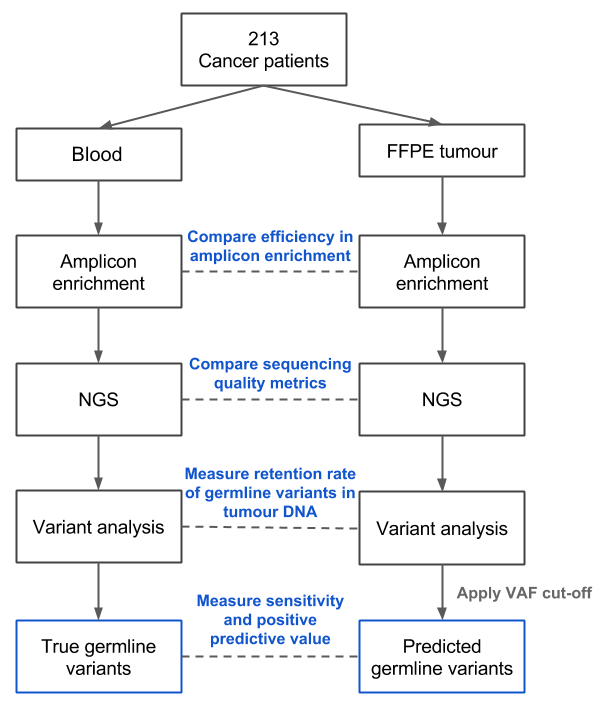
\includegraphics[scale=0.5]{study_design.png}
	\caption{Schematic description of study design and data analyses.}
	\label{fig:study_design}
\end{figure}

%%%%%%%%%%%%%%%%%%%%%%%%%%%%%%%%%%%%%%%%%%%%%%%%%%%%%%%%%%%%%%%%%%%%%
%%%%%%%%%%%%%%%%%%%%%%%%%%%%%%%%%%%%%%%%%%%%%%%%%%%%%%%%%%%%%%%%%%%%%

%%%%%%%%%%%%%%%%%%%%%%%%%%%%%%%%%%%%%%%%%%%%%%%%%%%%%%%%%%%%%%%%%%%%%%
\section{Patient samples}
\label{sec:Patientsamples}

Blood and FFPE tumour samples were acquired from 213 patients who provided informed consent for The OncoPanel Pilot (TOP) study (Human Research Ethics Protocol H14­-01212), a pilot study to optimize the OncoPanel, which is an amplicon-based targeted NGS panel for solid tumours. The TOP study also aims to assess the OncoPanel's application for guiding disease management and therapeutic intervention. One blood sample and four FFPE tumours were sequenced in duplicates, which resulted in 217 tumour-normal paired samples (434 sequencing libraries were included in our analyses). Patients in the TOP study are those with advanced cancers including CRC, lung cancer, melanoma, gastrointestinal stromal tumour (\acs{GIST}), and other cancers (\autoref{tbl:cancertypes}). The age of paraffin block for tumour samples ranges from 18 to 5356 days with a median of 274 days.

%%%%%%%%%%%%%%%%%%%%%%%%%%%%%%%%%%%%%%%%%%%%%%%%%%%%%%%%%%%%%%%%%%%%%%
%%%%%%%%%%%%%%%%%%%%%%%%%%%%%%%%%%%%%%%%%%%%%%%%%%%%%%%%%%%%%%%%%%%%%%
\begin{table}[H]
\caption{Distribution of cancer types in the TOP cohort.}
\label{tbl:cancertypes}
\centering
      \begin{tabular}{lccc}
        \hline
        Cancer Type & Number of Cases & Percentage (\%) \\ \hline
        Colorectal & 97 & 46 \\
        Lung & 60 & 28 \\
        Melanoma & 18 & 8 \\
				Other\textsuperscript{$\dagger$} & 16 & 8 \\
				GIST & 7 & 3 \\
				Sarcoma & 4 & 2 \\
				Neuroendocrine & 4 & 2 \\
				Cervical & 2 & 0.9 \\
				Ovarian & 2 & 0.9 \\
				Breast & 2 & 0.9 \\
				Unknown & 1 & 0.5 \\ \hline
      \end{tabular} \\
			\vspace{0.5cm}
\justify
{\small \textsuperscript{$\dagger$}This category includes thyroid, peritoneum, Fallopian tube, gastric, endometrial, squamous cell carcinoma, anal, salivary gland, peritoneal epithelial mesothelioma, adenoid cystic carcinoma, pancreas, breast, gall bladder, parotid epithelial myoepithelial carcinoma, carcinoid, and small bowel cancers.}
\end{table}

%%%%%%%%%%%%%%%%%%%%%%%%%%%%%%%%%%%%%%%%%%%%%%%%%%%%%%%%%%%%%%%%%%%%%%
\section{Sample preparation, library construction, and Illumina sequencing}
\label{sec:Samplepreparation,libraryconstruction,andIlluminasequencing}

Genomic DNA was extracted from blood and FFPE tumour samples using the Gentra Autopure LS DNA preparation platform and QIAamp DNA FFPE tissue kit (Qiagen, Hilden, Germany), respectively. The extracted DNA was sheared according to a previously described protocol \cite{Bosdet2013} to obtain approximate sizes of 3 kb followed by PCR primer merging, amplification of target regions, and adapter ligation using the Thunderstorm NGS Targeted Enrichment System (RainDance Technologies, Lexington, MA) as per manufacturer's protocol. Barcoded amplicons were sequenced with the Illumina MiSeq system for paired end sequencing with a v2 250-bp kit (Illumina, San Diego, CA).

%%%%%%%%%%%%%%%%%%%%%%%%%%%%%%%%%%%%%%%%%%%%%%%%%%%%%%%%%%%%%%%%%%%%%
\newpage
\section{OncoPanel (Amplicon-based targeted sequencing panel for solid tumours)}
\label{sec:OncoPanel}

The OncoPanel assesses coding exons and clinically relevant hotpots of 15 cancer-related genes and six PGx genes that can predict risk of developing chemotherapy-induced toxicity. Primers were designed by RainDance Technologies (Lexington, MA) using the GRCh37/hg19 human reference genome to generate 416 amplicons between 56 bp and 288 bp in size, which interrogate $\sim$20 kb of target bases. Complete list of genes and gene reference models for the OncoPanel is presented in \autoref{tbl:genemodel}, whereas OncoPanel target regions and amplicons are presented in \autoref{tbl:amplicons_target_regions}.

\normalsize
\begin{table}[H]
    \caption{Gene reference models for HGVS nomenclature of OncoPanel genes.}
    \label{tbl:genemodel}
    \centering
    \begin{tabular}{llll}
    \hline
    Gene & Protein & Reference Model \\
    \hline
    \multicolumn{3}{l}{\textit{Cancer-related}}
    \\
    AKT1 & Protein kinase B & NM\_001014431.1 \\
    ALK & Anaplastic lymphoma receptor tyrosine kinase & NM\_004304.3 \\
    BRAF & Serine/threonine-protein kinase B-Raf & NM\_004333.4 \\
    EGFR & Epidermal growth factor receptor & NM\_005228.3 \\
    HRAS & GTPase HRas & NM\_005343.2 \\
    MAPK1 & Mitogen-activated protein kinase 1 & NM\_002745.4 \\
    MAP2K1 & Mitogen-activated protein kinase kinase 1 & NM\_002755.3 \\
    MTOR & Serine/threonine-protein kinase mTOR & NM\_004958.3 \\
    NRAS & Neuroblastoma RAS viral oncogene homolog & NM\_002524.3 \\
    PDGFRA & Platelet-derived growth factor receptor alpha & NM\_006206.4 \\
    PIK3CA & Phosphatidylinositol-4,5-bisphosphate 3-kinase catalytic subunit alpha & NM\_006218.2 \\
    PTEN & Phosphatase and tensin homolog & NM\_000314.4 \\
    STAT1 & Signal transducer and activator of transcription 1 & NM\_007315.3 \\
    STAT3 & Signal transducer and activator of transcription 3 & NM\_139276.2 \\
    TP53 & Tumor protein P53 & NM\_000546.5 \\
    \\
    \multicolumn{3}{l}{\textit{Pharmacogenomics}}
    \\
    DPYD & Dihydropyrimidine dehydrogenase & NM\_000110.3 \\
    GSTP1 & Glutathione S-rransferase pi 1 & NM\_000852.3 \\
    MTHFR & Methylenetetrahydrofolate reductase & NM\_005957.4 \\
    TYMP & Thymidine phosphorylase & NM\_001113755.2 \\
    TYMS & Thymidylate synthetase & NM\_001071.2 \\
    UGT1A1 & Uridine diphosphate (UDP)-glucuronosyl transferase 1A1 & NM\_000463.2\\
    \hline
    \end{tabular}
\end{table}


%%%%%%%%%%%%%%%%%%%%%%%%%%%%%%%%%%%%%%%%%%%%%%%%%%%%%%%%%%%%%%%%%%%%%%
\section{Variant calling pipeline}
\label{sec:Variantcallingpipeline}

\subsection{Read alignment and variant calling}

Reads that passed the Illumina Chastity filter were aligned to the hg19 human reference genome using the \acs{BWA} mem algorithm (version 0.5.9) with default parameters, and the alignments were processed and converted to the BAM format using SAMtools (version 0.1.18). The SAMtools \texttt{mpileup} function \texttt{(samtools mpileup -BA -d 500000 -L 500000 -q 1)} was used to generate pileup files for all target bases followed by variant calling with the VarScan2 \texttt{mpileup2cns} (version 2.3.6) function with parameter thresholds of VAF $\geq$ 10\% and Phred-scaled BAQ score $\geq$ 20 \texttt{(--min-var-freq 0.1 --min-avg-qual 20 --strand-filter 0 --p-value 0.01 --output-vcf --variants)}.

Four genomic positions at which the hg19 human reference genome contains potential risk alleles were identified (\autoref{tbl:potential_risk_alleles}). Hence, patients homozygous for these four risk alleles would not be identified by our standard variant calling procedure. For these four genomic sites, our method for variant calling was modified to provide calls for every patient in the cohort. The VarScan2 \texttt{mpileup2cns} function with parameter thresholds of VAF $\geq$ 25\%, VAF to call homozygote $\geq$ 90\%, BAQ score $\geq$ 20, and fraction of variant reads from each strand $\geq$ 0.1 \texttt{(--min-var-freq 0.25 --min-freq-for-hom 0.9 --min-avg-qual 20 --strand-filter 1 \\--p-value 0.01 --output-vcf)} was used. Next, allelic statuses were re-assigned, in which wild type calls were re-assigned as homozygous variants, while homozygous variants were re-assigned as wild type calls. Corrections to the VAFs of these four genomic sites were also made to ensure that the VAFs reflect percentage of reads with the risk alleles.

%%%%%%%%%%%%%%%%%%%%%%%%%%%%%%%%%%%%%%%%%%%%%%%%%%%%%%%%%%%%%%%%%%%%%%
%%%%%%%%%%%%%%%%%%%%%%%%%%%%%%%%%%%%%%%%%%%%%%%%%%%%%%%%%%%%%%%%%%%%%%

\begin{longtable}{p{0.08\linewidth}|p{0.05\linewidth}p{0.1\linewidth}p{0.13\linewidth}p{0.16\linewidth}p{0.2\linewidth}}
    \caption{Potential risk alleles in the hg19 human reference genome within the target regions of the OncoPanel.}
    \label{tbl:potential_risk_alleles}
        \\
        \hline
        Gene & Chr & Pos & Risk Allele & dbSNP ID & HGVS\textsuperscript{*}
				\\
				\hline
        DPYD & chr1 & 98348885 & C & rs1801265 & p.Cys29Arg c.85T$>$C
        \\
        MTOR & chr1 & 11205058 & G & rs386514433; rs1057079 & p.Ala1577Ala c.4731A$>$G
        \\
        & chr1 & 11288758 & C & rs1064261 & p.Asn999Asn c.2997T$>$C
        \\
        TP53 & chr17 & 7579472 & C & rs1042522 & p.Arg72Pro c.215G$>$C
        \\
				\hline
\end{longtable}
\textsuperscript{*}Description of sequence variants according to the HGVS recommendations.

%%%%%%%%%%%%%%%%%%%%%%%%%%%%%%%%%%%%%%%%%%%%%%%%%%%%%%%%%%%%%%%%%%%%%%
%%%%%%%%%%%%%%%%%%%%%%%%%%%%%%%%%%%%%%%%%%%%%%%%%%%%%%%%%%%%%%%%%%%%%%

\subsection{Variant filtering}

Variant calls were filtered using the VarScan2 \texttt{fpfilter} function with fraction of variant reads from each strand $\geq$ 0.1 and default thresholds for other parameters (\autoref{tbl:varscan_fpfilter_parameters}). The VarScan2 \texttt{fpfilter} removed 247 low quality variants. Seventy germline variants in the blood were also excluded from our analysis because these variants in the tumours were filtered by the VarScan2 \texttt{fpfilter}. There were also 16 risk allele calls in tumour samples that did not pass the strand filter, causing the removal of 10 risk allele calls in the blood samples from our evaluation. Overall, a total of 343 calls were excluded by the VarScan2 \texttt{fpfilter} and strand filter. Manual inspection was performed for a subset of variants, including variants detected within primer regions and in PGx genes, using the Intergrative Genomics Viewer (IGV, version 2.3). This resulted in the removal of 500 spurious calls, which stemmed from software bugs, sequencing artifacts, primer masking, and primer artifacts (\autoref{tbl:spurious_calls}). Eleven low coverage calls ($\leq$ 100x) were also excluded from our analysis. Implementation of this filtering pipeline reduced the raw variant output of 5288 calls from 217 paired tumour-blood samples (434 sequencing libraries) to 4434 calls (\autoref{fig:variant_pipeline}B).

%%%%%%%%%%%%%%%%%%%%%%%%%%%%%%%%%%%%%%%%%%%%%%%%%%%%%%%%%%%%%%%%%%%%%%
%%%%%%%%%%%%%%%%%%%%%%%%%%%%%%%%%%%%%%%%%%%%%%%%%%%%%%%%%%%%%%%%%%%%%%

\begin{table}[H]
\caption{Thresholds for parameters of VarScan2 \texttt{fpfilter} used for filtering raw variant output.}
\label{tbl:varscan_fpfilter_parameters}
\centering
      \begin{tabular}{p{0.3\linewidth}p{0.56\linewidth}cp{0.1\linewidth}}
        \hline
        Parameter & Description & Threshold
				\\
				\hline
				\texttt{--min-var-count} & Min number of var-supporting reads & 4
				\\
        \texttt{--min-var-count-lc} & Min number of var-supporting reads when depth below somaticPdepth & 2
        \\
        \texttt{--min-var-freq} & Min variant allele frequency & 0.1
				\\
        \texttt{--max-somatic-p} & Max somatic p-value & 0.05
				\\
        \texttt{--max-somatic-p-depth} & Depth required to test max somatic p-value & 10
				\\
        \texttt{--min-ref-readpos} & Min average read position of ref-supporting reads & 0.1
				\\
        \texttt{--min-var-readpos} & Min average read position of var-supporting reads & 0.1
				\\
        \texttt{--min-ref-dist3} & Min average distance to effective 3' end of ref reads & 0.1
				\\
        \texttt{--min-var-dist3} & Min average distance to effective 3' end of variant reads & 0.1
				\\
        \texttt{--min-strandedness} & Min fraction of variant reads from each strand & 0.1
				\\
        \texttt{--min-strand-reads} & Min allele depth required to perform the strand tests & 5
				\\
        \texttt{--min-ref-basequal} & Min average base quality for ref allele & 15
				\\
        \texttt{--min-var-basequal} & Min average base quality for var allele & 15
				\\
        \texttt{--min-ref-avgrl} & Min average trimmed read length for ref allele & 90
				\\
        \texttt{--min-var-avgrl} & Min average trimmed read length for var allele & 90
        \\
        \texttt{--max-rl-diff} & Max average relative read length difference (ref - var) & 0.25
        \\
        \texttt{--max-ref-mmqs} & Max mismatch quality sum of ref-supporting reads & 100
        \\
        \texttt{--max-var-mmqs} & Max mismatch quality sum of var-supporting reads & 100
        \\
        \texttt{--max-mmqs-diff} & Max average mismatch quality sum (var - ref) & 50
        \\
        \texttt{--min-ref-mapqual} & Min average mapping quality for ref allele & 15
        \\
        \texttt{--min-var-mapqual} & Min average mapping quality for var allele & 15
        \\
        \texttt{--max-mapqual-diff} & Max average mapping quality (ref - var) & 50
        \\
				\hline
      \end{tabular}
\end{table}

%%%%%%%%%%%%%%%%%%%%%%%%%%%%%%%%%%%%%%%%%%%%%%%%%%%%%%%%%%%%%%%%%%%%%%
%%%%%%%%%%%%%%%%%%%%%%%%%%%%%%%%%%%%%%%%%%%%%%%%%%%%%%%%%%%%%%%%%%%%%%

\subsection{Variant annotation and interpretation}

SnpEff (version 4.2) was used for effect prediction, and the SnpSift package in SnpEff was used to annotate variants with databases such as dbSNP (b138), COSMIC (version 70), 1000 Genomes Project, and \acs{ExAC} (release 0.3) for interpretation. Clinical significance reported by the ClinVar database and literature review were also used for variant interpretation.

%%%%%%%%%%%%%%%%%%%%%%%%%%%%%%%%%%%%%%%%%%%%%%%%%%%%%%%%%%%%%%%%%%%%%%
%%%%%%%%%%%%%%%%%%%%%%%%%%%%%%%%%%%%%%%%%%%%%%%%%%%%%%%%%%%%%%%%%%%%%%

\newpage
\begin{longtable}{p{0.08\linewidth}p{0.05\linewidth}p{0.1\linewidth}p{0.04\linewidth}p{0.04\linewidth}p{0.6\linewidth}}
    \caption{Spurious variants removed by the variant filtering pipeline.}
    \label{tbl:spurious_calls}
        \\
        \hline
        Gene & Chr & Pos & Ref & Alt & Reason
				\\
				\hline
				KIT & chr4 & 55599268 & C & T & Variant masked by primer in FFPE specimen
				\\
        MAPK1 & chr22 & 22162126 & A & G & Variant masked by primer in FFPE specimen
        \\
        MTOR & chr1 & 11186783 & G & A & Sequencing artifact within primer region
        \\
        MTOR & chr1 & 11190646 & G & A & Variant masked by primer in FFPE specimen
        \\
        TYMP & chr22 & 50964446 & A & T & Poor target region, alignment of different sized amplicons
        \\
        TYMP & chr22 & 50964862 & A & T & Poor target region, alignment of different sized amplicons
        \\
        TYMS & chr18 & 673449 & G & C & VarScan2 bug after chr18:673443 c.*447\_*452delTTAAAG
        \\
        UGT1A1 & chr2 & 234668879 & CAT & C & Sequencing artifact at AT repeats in promoter
        \\
        UGT1A1 & chr2 & 234668881 & T & TAC & VarScan2 bug after AT insertion in promoter
        \\
				\hline
\end{longtable}

%%%%%%%%%%%%%%%%%%%%%%%%%%%%%%%%%%%%%%%%%%%%%%%%%%%%%%%%%%%%%%%%%%%%%%
%%%%%%%%%%%%%%%%%%%%%%%%%%%%%%%%%%%%%%%%%%%%%%%%%%%%%%%%%%%%%%%%%%%%%%

\begin{figure}[H]
\centering
	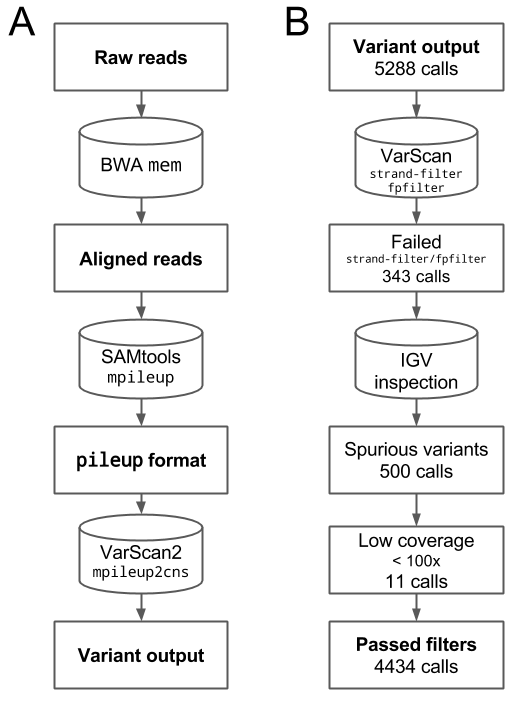
\includegraphics[scale=0.55]{variant_pipeline3.png}
	\caption{Pipelines for (A) variant calling and (B) filtering.}
	\label{fig:variant_pipeline}
\end{figure}

%%%%%%%%%%%%%%%%%%%%%%%%%%%%%%%%%%%%%%%%%%%%%%%%%%%%%%%%%%%%%%%%%%%%%%
\newpage
\section{Sequence analysis}
\label{sec:Sequenceanalysis}

A custom Python script was used to process BAM files to quantify the number of on-target aligned (reads that map to target regions), off-target aligned (reads that map to hg19 but not target regions), and unaligned reads with a Phred-scaled mapping quality (\acs{MAPQ}) score $\geq$ 10. Unaligned reads were also screened against microbial sequences, including viruses, archaea, bacteria, and fungi, to ensure that samples do not contain significant amount of microbial contaminants. Coverage depth for target bases with MAPQ $\geq$ 1 and BAQ $\geq$ 20 was obtained using bam-readcount (https://github.com/genome/bam-readcount). To measure coverage depth of amplicons, the SAMtools \texttt{view} function was used to filter for reads with MAPQ $\geq$ 1 \texttt{(samtools view -b -q 1)} followed by the bedtools \texttt{intersect} function (version 2.25.0) to quantify the number of reads that overlap with amplicon positions \texttt{(intersect -a \$AMPLICON\_POSITIONS -b \$BAM\_FILE -f 0.95 -r -c)}.

Per-base metrics generated using bam-readcount were also used for assessment of sequence artifacts. A custom R script was used to count and categorize the different groups of base changes (i.e. C$>$T/G$>$A, A$>$G/T$>$C, C$>$A/G$>$T, A$>$C/T$>$G, C$>$G/G$>$C, and A$>$T/T$>$A). Unless stated otherwise, analysis of sequence artifacts excludes true variants identified by our VarScan2 variant calling pipeline and base changes with VAF $<$ 1\%, which are considered sequencing errors. All statistical analyses and data visualization were performed using the R statistical software package (version 3.3.2) and associated open-source packages.

%%%%%%%%%%%%%%%%%%%%%%%%%%%%%%%%%%%%%%%%%%%%%%%%%%%%%%%%%%%%%%%%%%%%%%
\section{Application of VAF thresholds to separate germline alterations from somatic mutations}
\label{sec:ApplicationofVAFthresholdstoseparategermlinealterationsfromsomaticmutations}

Variants in the tumours that passed our filtering criteria were subjected to VAF thresholds between 10--45\%. At each VAF cut-off, variants that were not filtered out were considered predicted germline variants. Given that all tumour samples have matched blood samples, true positives were identified as predicted germline variants that overlap with variants in the blood (\autoref{fig:tpfptnfn}). Conversely, false negatives were identified as variants that were filtered out by the VAF cut-off (predicted as somatic), but were present in the blood samples. Sensitivity at each VAF threshold was calculated by dividing the number of true positives with the sum of true positives and false negatives. Because predicted germline variants will be referred to follow-up germline testing, positive predictive values (\acs{PPV}s) were calculated at each VAF cut-off to evaluate precision of our approach. False positives were identified as predicted germline variants that were absent in the blood, and PPV was calculated by dividing the number of true positives with the sum of true positives and false positives.

%%%%%%%%%%%%%%%%%%%%%%%%%%%%%%%%%%%%%%%%%%%%%%%%%%%%%%%%%%%%%%%%%%%%%%
%%%%%%%%%%%%%%%%%%%%%%%%%%%%%%%%%%%%%%%%%%%%%%%%%%%%%%%%%%%%%%%%%%%%%%

\begin{figure}[H]
\centering
	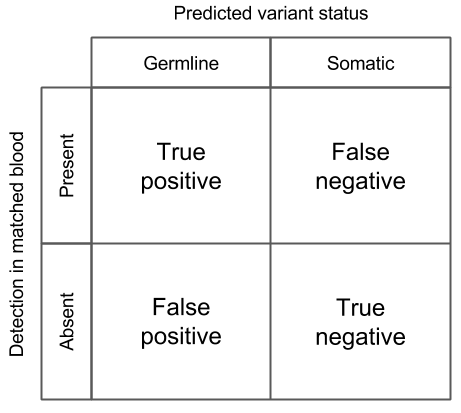
\includegraphics[scale=0.55]{tpfptnfn.png}
	\caption{2x2 contingency table for determination of true positive, false positive, true negative, and false negative variant calls in tumour-only analyses.}
	\label{fig:tpfptnfn}
\end{figure}


%%%%%%%%%%%%%%%%%%%%%%%%%%%%%%%%%%%%%%%%%%%%%%%%%%%%%%%%%%%%%%%%%%%%%%

\endinput


%    3. Results
%% The following is a directive for TeXShop to indicate the main file
%%!TEX root = diss.tex

\chapter{Results}
\label{ch:Results}

%%%%%%%%%%%%%%%%%%%%%%%%%%%%%%%%%%%%%%%%%%%%%%%%%%%%%%%%%%%%%%%%%%%%%%
\section{Frequency of germline and somatic variants}
\label{sec:Frequencyofgermlineandsomaticvariants}

\begin{table}[htb]
\caption{Frequency of germline and somatic variants detected in the tumours of 213 patients in the TOP cohort.}\label{metrics}
\centering
\begin{tabular}{lcclcl}
        \hline
        Gene & Germline & Pathogenic Germline && Somatic \\
				 & (N Patients) & (N Patients) && (N Patients) \\
				\hline
				\multicolumn{1}{l}{\textit{Cancer predisposing}}
				&
				\multicolumn{2}{l}{ }
				&&
				\multicolumn{1}{l}{} \\
				\hline
				AKT1 & 0 & 0 && 2 (2) \\
				\arrayrulecolor{evagrey}\hline
				ALK & 1 (1) & 1 (1) && 2 (1) \\
				\hline
				BRAF & 0 & 0 && 18 (17) \\
				\hline
				EGFR & 170 (164) & 5 (5) && 31 (24) \\
				\hline
				HRAS & 0 & 0 && 1 (1) \\
				\hline
				MAP2K1 & 0 & 0 && 2 (2) \\
				\hline
				MAPK1 & 17 (17) & 3 (3) && 3 (2) \\
				\hline
				MTOR & 763 (213) & 6 (6) && 71 (30) \\
				\hline
				NRAS & 0 & 0 && 8 (8) \\
				\hline
				PDGFRA & 242 (185) & 0 && 8 (4) \\
				\hline
				PIK3CA & 0 & 0 && 15 (4) \\
				\hline
				PTEN & 0 & 0 && 1 (1) \\
				\hline
				STAT1 & 54 (51) & 1 (1) && 7 (6) \\
				\hline
				STAT3 & 10 (10) & 4 (4) && 16 (11) \\
				\hline
				TP53 & 189 (184) & 2 (2) && 131 (109) \\
				\arrayrulecolor{black}\hline
				\\
				\multicolumn{1}{l}{\textit{Pharmacogenomics}}
				&
				\multicolumn{2}{l}{ }
				&&
				\multicolumn{1}{l}{} \\
				\arrayrulecolor{black}\hline
				DPYD & 271 (212) & 1 (1) && 1 (1) \\
				\arrayrulecolor{evagrey}\hline
				GSTP1 & 106 (106) & 0 && 0 \\
				\hline
				MTHFR & 209 (177) & 0 && 0 \\
				\hline
				TYMP & 81 (76) & 2 (2) && 18 (13)\\
				\hline
				TYMS & 131 (131) & 0 && 0 \\
				\hline
				UGT1A1 & 96 (96) & 0 && 1 (1) \\
				\arrayrulecolor{black}\hline \\
				\\
				Total & 2396 (213*) & 25 (23*) && 431 (180) \\
				\arrayrulecolor{black}\hline
      \end{tabular}
\end{table}

%%%%%%%%%%%%%%%%%%%%%%%%%%%%%%%%%%%%%%%%%%%%%%%%%%%%%%%%%%%%%%%%%%%%%%
\section{Variant Allele Frequency Thresholds Can Maximize Sensitivity and Positive Predictive Value of Germline Variant Calling in Tumours}
\label{sec:VariantAlleleFrequencyThresholdsCanMaximizeSensitivityandPositivePredictiveValueofGermlineVariantCallinginTumours}


%    4. Discussion and conclusion
%% The following is a directive for TeXShop to indicate the main file
%%!TEX root = diss.tex

\chapter{Discussion and Conclusion}
\label{ch:Discussionandconclusion}


%    2. Main body
% Generally recommended to put each chapter into a separate file
%\include{relatedwork}
%\include{model}
%\include{impl}
%%% The following is a directive for TeXShop to indicate the main file
%%!TEX root = diss.tex

%%%%%%%%%%%%%%%%%%%%%%%%%%%%%%%%%%%%%%%%%%%%%%%%%%%%%%%%%%%%%%%%%%%%%%
\chapter{Discussion}
\label{ch:Discussion}
%%%%%%%%%%%%%%%%%%%%%%%%%%%%%%%%%%%%%%%%%%%%%%%%%%%%%%%%%%%%%%%%%%%%%%

Genomic analyses of tumours can reveal druggable somatic mutations, as well as clinically relevant germline alterations that are beneficial to patients and their family members \cite{Meric-Bernstam2016, Schrader2015, Jones2015a}. While sequencing of tumour-normal pairs can enable differentiation between germline and somatic variants, matched normal samples are often not obtained in clinical practice. Moreover, FFPE tumour tissues represent another challenge in clinical genomics. Formalin fixation damages nucleic acid through fragmentation and cytosine deamination, which affect molecular testing with FFPE DNA \cite{Do2015a, Kim2017, Ofner2017, Oh2015, Wong2013, Wong2014, Sikorsky2007}. Hence, usability of FFPE DNA for germline testing and approaches to discriminate between germline and somatic variants in tumour-only analyses must be evaluated. These assessments would facilitate optimization of workflows to identify potential germline alterations using clinical tumour sequencing.

In this study, we retrospectively analyzed targeted sequencing data from tumour and matched blood specimens of 213 cancer patients. Our findings demonstrated that DNA fragmentation and cytosine deamination were common forms of DNA damage in FFPE specimens. While the impact of formalin fixation on amplicon enrichment and sequencing results was detectable, we determined that these discrepancies were either technically negligible or could be minimized using appropriate methods. We also found that the majority of germline alterations identified in blood using our panel test were present with the same allelic statuses in FFPE tumours. This implies that a high proportion of germline genetic changes are retained in the tumour genome, demonstrating the reliability of using tumour DNA for germline variant calling. Finally, we assessed the application of VAF threshold to delineate germline and somatic variants in tumour-only analyses. We reported that a VAF cut-off of 30\% would correctly identify 94\% of germline alterations, while erroneously submit 10\% of false positives, which are somatic mutations, for follow-up germline testing. Because our gene panel and patient cohort are relatively small, we were only able to identify germline variants that are predictive of drug response. However, we surmised that application of this VAF cut-off could be expanded to predict the statuses of pathogenic germline variants such as alterations in \textit{BRCA} genes.

\subsection{Effects of formalin-induced DNA damage on sequencing metrics are minor and technically insignificant}

Several studies have reported findings that are consistent with our assessment of formalin-induced DNA damage in FFPE specimens. To assess the usability of FFPE DNA for germline testing, we compared efficiency in amplicon enrichment and sequencing results of FFPE DNA to blood, which is a gold standard for germline testing. We noted lower efficiency in amplicon enrichment in FFPE DNA, with a more pronounced decrease in coverage depth for longer amplicons in the panel. Similarly, Shi et al. \cite{Shi2002}, Didelot et al. \cite{Didelot2013}, and Wong et al. \cite{Wong2013} demonstrated that shorter amplicons gave rise to better PCR amplification success in FFPE DNA, indicating the presence of fragmentation damage, which yields template DNA of shorter fragment lengths. While we observed comparable proportion of on-target aligned reads between FFPE and blood DNA, there were minor discrepancies in coverage depth and uniformity of target bases in FFPE DNA. Various groups have also reported disparities in coverage depth and uniformity in FFPE DNA when compared to DNA extracted from either fresh frozen or unfixed specimens \cite{Wong2013, Betge2015, Spencer2013}. Additionally, Wong et al. \cite{Wong2014} and Didelot et al \cite{Didelot2013} showed inverse correlations between coverage depth and the degree of DNA fragmentation in FFPE DNA, suggesting that formalin-induced fragmentation damage could be accountable for such discrepancies in sequencing results. Although we detected differences in sequencing results between FFPE and blood DNA, we concluded that these effects were minor and technically insignificant. As for the discrepancy in amplicon enrichment, shorter amplicons can be designed to circumvent the drawback of fragmentation damage in FFPE samples.

\subsection{Impact of artifactual base changes on germline variant calling can be mitigating by applying a VAF cut-off}

Cytosine deamination is a major cause of sequence artifacts in formalin-fixed specimens \cite{Wong2014, Do2012, Oh2015, Spencer2013, Do2013, Kim2017, Chen2014}. Herein, we observed increased C$>$T/G$>$A artifacts in FFPE DNA compared to blood. Artifactual C$>$T/G$>$A changes are formed by incorporation of adenines in the complementary DNA strand at uracil lesions generated by deamination of cytosines \cite{Do2015a}. When measuring frequency of sequence artifacts at different allele frequency ranges, Wong et al. \cite{Wong2014} reported higher C$>$T/G$>$A transitions at a lower allele frequency range (1--10\% \textit{vs.} 10--25\%). This finding led us to compare the fraction of base changes at different allele frequency ranges, including 1--10\%, 10--20\%, and 20--30\%. Indeed, we observed a substantial increase in C$>$T/G$>$A within the 1--10\% allele frequency range. Considering that our goal is to predict germline status, disproportionate base changes between FFPE and blood DNA within these allele frequency ranges suggest that germline calls should be made at $>$ 30\% VAF to avoid false positives that could either arise from true somatic mutations or FFPE artifacts. We were unable to separate FFPE artifacts from low-allelic-fraction somatic mutations within these allele frequency ranges due to the lack of matched fresh frozen or unfixed tumour tissues. Nevertheless, somatic mutations can occur at VAFs that deviate significantly from a diploid zygosity (i.e. heterozygous variant should have VAF close to 50\%, whereas homozygous variant should have VAF close to 100\%) because of low tumour content or tumour heterogeneity \cite{Kim2017a, Xu2017, Carrot-Zhang2016, Tian2015, Cai2016}. Therefore, further workflow optimization should be performed for the purpose of identifying clinically relevant somatic mutations in the tumour genome. A method to reduce sequence artifacts caused by cytosine deamination is through treatment with uracil-DNA glycosylase (UDG) before sequencing. UDG is an enzyme capable of depleting uracil lesions in DNA, giving rise to abasic sites. During PCR amplification, cytosine bases are restored at abasic sites by using the complementary DNA strand as template, which consists of guanine bases opposite of the uracil lesions \cite{Do2015a}. Several studies showed that pre-treatment of FFPE DNA with UDG can markedly reduce C$>$T/G$>$A sequence artifacts \cite{Do2013, Kim2017, Do2012}. However, this approach cannot correct sequence artifacts at CpG dinucleotides because these cytosines are typically methylated, and deamination of 5-methyl cytosines generates thymines instead uracil bases, which are resistant to UDG repair \cite{Do2013}.

\subsection{Sequence artifacts other than those caused by cytosine deamination are detected}

We also observed elevated levels of A$>$G/T$>$C artifacts in FFPE DNA, albeit to a lesser extent compared to C$>$T/G$>$A artifacts. Likewise, Wong et al. \cite{Wong1998} reported that 35\% of sequence artifacts in Sanger sequencing of the \textit{BRCA1} gene were A$>$G/T$>$C nucleotide changes. We speculate that increase in A$>$G/T$>$C artifacts is caused by deamination of adenine to generate hypoxanthine, which forms base pairs with cytosine instead of thymine. This results in transformation of A-T base pairs to G-C base pairs. Deamination of adenine to hypoxanthine can be catalyzed by an acidic environment \cite{Wang2010}, which can arise in FFPE specimens because formaldehyde can be oxidized to generate formic acid \cite{Do2015a}. Acidic conditions also promotes depurination, creating abasic sites. Many DNA polymerases selectively incorporate adenines across abasic sites, while guanines and small deletions are integrated in fewer cases \cite{Heyn2010}. Despite statistically insignificant, we observed a subset of FFPE specimens with higher fractions of C$>$A/G$>$T artifacts. These artifactual changes could have resulted from depurination of guanines, followed by incorporation of adenines by DNA polymerase in the complementary strand, which alters G-C base pairs to A-T base pairs. Heyn et al. \cite{Heyn2010} reported that DNA polymerases demonstrated varying bypass rates at abasic sites. For instance, AmpliTaq Gold, \textit{Pfu}, and Platinum Taq HiFi extended across lower frequency of abasic sites compared to Platinum Taq, \textit{Bst} and \textit{Sso}-Dpo4 ($<$34\% \textit{vs.} $>$77\%) \cite{Heyn2010}. Thus, selection of a high fidelity DNA polymerase could lessen these forms of sequence artifacts. Costello et al. \cite{Costello2013} discovered that C$>$A/G$>$T artifacts can also occur due to oxidation of DNA during the shearing process, converting guanines to 8-oxoguanine lesions. This conversion is highly dependent on the surrounding 5' and 3' bases of the guanine, in which guanines within GGC are the most susceptible to oxidation. 8-oxoguanine can form base pairs with cytosine and adenine, and mispairing with adenine would give rise to artifactual C$>$A/G$>$T transversions. However, this was not the cause of C$>$A/G$>$T artifacts in our data because both blood and FFPE DNA were sheared, and we did not observe simultaneous C$>$A/G$>$T increments in both specimen types compared to other types of base changes.

\subsection{Storage time of FFPE blocks correlates with the extent of formalin-induced DNA damage}

Ludyga et al. \cite{Ludyga2012} demonstrated that long-term storage of FFPE blocks led to increased DNA fragmentation, producing shorter template DNA for PCR amplification. Furthermore, Carrick et al. \cite{Carrick2015} showed that increased storage time of FFPE blocks affects sequencing coverage and depth in NGS data. These findings are in agreement with our results, in which we found negative associations between age of paraffin blocks and efficiency in amplicon enrichment, coverage depth of target bases, and percentage of on-target aligned reads. As well, we observed a positive correlation between age of paraffin blocks and fraction of C$>$T/G$>$A artifacts, an outcome of stochastic enrichment. Due to exposure to environmental conditions, older FFPE blocks tend to produce increasingly fragmented DNA, which results in lower amounts of amplifiable DNA. Consequently, there is a higher chance of amplifying template DNA with sequence artifacts caused by formalin, yielding increased frequency of artifactual nucleotide changes in older FFPE specimens \cite{Wong2014}. These results demonstrating the correlations between storage time of paraffin blocks and sequencing variables suggest that if multiple FFPE blocks are available, the specimen with the shorter storage time should be selected for molecular testing. However, clinical specimens are often limited, making sample selection a rare option in the diagnostic setting. As such, other approaches to eliminate sequence artifacts should be considered such as application of molecular barcodes and hybridization-capture enrichment, which allow tracking of DNA templates \cite{Eijkelenboom2016, Samorodnitsky2015, Peng2015, Wong2013}. This would enable detection of variants that are only supported by the same template DNA, indicating a higher chance that these variants are sequence artifacts and should be interpreted with caution.

\subsection{Germline variants are highly retained in the tumour genome}

Various groups have identified clinically significant germline alterations through analyzing tumour genomes \cite{Schrader2015, Meric-Bernstam2016, Jones2015a, WcWhinney2009}. Schrader et al. \cite{Schrader2015} reported that potential pathogenic germline variants in cancer-predisposing genes were conserved in the tumours of 91.9\% of patients in their study cohort (182 of 198 patients), whereas 21.4\% of these patients (39 of 182 patients) demonstrated LOH or other forms of mutations in the remaining wild type allele. We found that 93.8\% of germline alterations identified in the blood were retained in the tumour with the same allelic statuses, a finding that is in line with previous work. This suggests that tumour DNA could be a reliable substrate for detecting germline alterations, implying that a tumour-only sequencing protocol could be leveraged for pre-screening of germline variants before submission to downstream confirmatory testing. A framework as such could provide germline testing in a cost-effective manner because only selective patients (i.e. those with potential germline alterations that are clinically important) would require follow-up. We also identified discordant germline variants between blood and tumour DNA, which were caused by various reasons like LOH, low sequencing coverage ($<$ 100x), and loss of variant allele in the tumours. All tumour specimens in our study were formalin-fixed, therefore it is possible that DNA damage induced by formaldehyde exposure played a role in creating discordant germline variants. Variant discordance can also be caused by mutagenesis in the tumour, such as somatic CNVs in the region of the germline variant. For instance, Gross et al. \cite{Gross2013} showed a high prevalence of \textit{DPYD} CNVs in high-grade triple negative breast cancer, particularly in cases with copy number loss of the \textit{BRCA1} DNA-repair gene. The common fragile site FRA1E is located within the \textit{DPYD} gene and its stability is highly dependent on intact \textit{BRCA1} \cite{Arlt2004}. Hence, deficiency in \textit{BRCA1} protein would result in increased fragility of FRA1E, leading to genomic rearrangements in \textit{DPYD}. As germline variants in the \textit{DPYD} gene can predict susceptibility to 5-FU-related toxicity, somatic CNVs in \textit{DPYD} could affect the detection of these germline variants in tumour genomic sequencing.

\subsection{The use of VAF threshold is feasible for distinguishing between germline and somatic alterations in tumour-only analyses}

Although sequencing of tumour-normal pairs would enable accurate identification of germline and somatic variants, this approach is not routinely practice in clinical genomics due to inadequate funding and facilities to store additional specimens. Methods to distinguish between germline and somatic alterations in tumour-only analyses have been described by different groups \cite{Hiltemann2015, Jones2015a, Garofalo2016}. Hiltemann et al. \cite{Hiltemann2015} used a virtual normal that was assembled by aggregating whole-genome-sequenced normal samples from 931 healthy and unrelated individuals, whereas Jones et al. \cite{Jones2015a} resorted to using an unmatched normal sample and public databases such as dbSNP, 1000 Genomes Project, and COSMIC, as well as effect prediction tools. We leveraged the fact that the VAFs of somatic mutations typically deviate from 50\% and 100\% for heterozygous and homozygous variants, respectively, and employed VAF threshold to differentiate between variant statuses. Our approach managed to achieve high sensitivity and precision, therefore verifying the feasibility of using VAF threshold to differentiate between germline and somatic alterations in the absence of matched normal samples. The VAF threshold method takes advantage of genetic impurity and heterogeneity of tumours, which render the deviation of somatic VAFs from diploid zygosity. Jones et al. \cite{Jones2015a} discovered that performance of the VAF threshold approach was highly dependent on tumour purity. While the use of VAF threshold can correctly identify germline and somatic alterations in tumours with $<$ 50\% purity, this accuracy was not observed for specimens with higher tumour content. In fact, only 12.5\% of cancer-predisposing germline variants and an average of 48\% of somatic mutations were accurately predicted \cite{Jones2015a}. Unfortunately, pathologic estimation of tumour content was not available for our analyses. However, we speculate that the tumour specimens in our dataset are highly impure or heterogeneous, thereby contributing to the high sensitivity and precision attained by the VAF threshold approach. While there are bioinformatic algorithms available to infer clonality and impurity estimates of tumours, many of these methods require matched normal controls or are not compatible with targeted sequencing data \cite{Yadav2015}. Nevertheless, this information should be integrated into clinical pipelines to enhance the performance of using a VAF threshold approach to distinguish between germline and somatic alterations in the course of analyzing tumour genomes without matched normal samples.

\subsection{Limitations and future directions}

There are several limitations in our study. First, we did not manually review every single variant called by our pipeline. Only variants located within primer regions were manually inspected, while our variant filter also included common artifacts that were curated during clinical assessment. Hence, it is highly possible that sequence artifacts are present in our dataset, particularly low-allelic-fraction variants (i.e. $<$ 30\%) detected in the blood. These potentially artifactual variants account for 6\% of all germline variants identified in blood DNA, thereby compromising sensitivity of the VAF threshold method. Variant inspection using a genome browser is routinely conducted by genomic analysts in clinical practice to decrease the risk of reporting false positive results \cite{Strom2016, Garofalo2016}. However, manual review of variants was not implemented in our study because our analyses were focused on evaluating analytical validity instead of inferring clinical implications of the variants called. Moreover, the large number of variants in our study would be time-consuming and unfeasible for manual inspection. Our evaluation of the VAF threshold approach in differentiating between germline and somatic variants is favourable of the framework to implement initial screening for germline variants in clinical tumour sequencing before follow-up germline testing. The relatively small gene panel and cohort size of our study are caveats in drawing this conclusion. Although we were able to identify germline variants that can influence drug response, we did not report any pathogenic germline variants that are associated with cancer predisposition in our dataset. Hence, we can only speculate that our approach could be applicable to variants in cancer-predisposing genes. Studies that were able to identify pathogenic germline variants were performed with cohort sizes and gene panels that are substantially larger than ours. For instance, the study by Schrader et al. \cite{Schrader2015}, which revealed pathogenic germline variants in 16\% of patients, was performed in a cohort of 1566 patients and screened for 341 genes. To determine whether the VAF threshold method can be applied to detect genetic alterations linked to cancer susceptibility, further assessment which involves a larger patient cohort and surveying known cancer-predisposing genes must be carried out.

The present study addresses two problems faced by using tumour genomic sequencing to identify germline alterations: the widespread use of FFPE tumours and the lack of matched normal samples. Archival FFPE tissues remain a sizable resource for cancer genomic studies and clinical genomic sequencing. Thus, there is a need to understand the extent of the different forms of DNA damage induced by formalin. Our analyses not only provide insights on the impact of formalin-induced DNA damage on amplicon-based NGS data, but also help us devise guidelines to minimize these effects. Formalin fixation followed by paraffin embedding is an attractive method to preserve tissues for histologic assessment because it allows storage at ambient temperature, which reduces cost that could be incurred by maintaining freezers required for fresh-frozen samples. Yet, many studies, including ours, have indicated the side effects of the formaldehyde exposure on nucleic acid \cite{Do2015a, Kim2017, Ofner2017, Oh2015, Wong2013, Wong2014, Sikorsky2007}. Instead of investing efforts into mitigating these side effects, a potential solution is to transition from the use of formalin to the UMFIX (Sakura Finetek USA, Inc.) fixative, which is capable of preserving both cellular morphology for pathologic review and macromolecules, including DNA \cite{Vincek2003}. Most clinical laboratories conduct tumour-only sequencing and apply approaches to distinguish between germline and somatic alterations. Without matched normal samples, interpretation of variants becomes complicated. Jones et al. \cite{Jones2015a} and Garofalo et al. \cite{Garofalo2016} concluded that sequencing of tumour-normal pairs is the best practice to accurately identify variant statuses. For a center to provide this service, it must be equipped to collect, analyze, and report germline findings. This includes establishing appropriate pre-test and post-test counseling, protocols to secure patient consent and manage variant of uncertain significance, and frameworks to communicate results that may implicate the patients' relatives. While various groups recommend the sequencing of tumour-normal pairs, some centers simply do not have the funding or infrastructure to implement this as a standard practice. Furthermore, the American College of Medical Genetics and Genomics (\acs{ACMG}) recommended that clinical laboratories report incidental variants in 56 genes that are associated with disease risk in DNA derived from germline samples, including matched normal samples that only serve the purpose of subtracting germline variants to identify somatic mutations in tumours \cite{Green2013}. Interrogation of these genes suggested by the ACMG guidelines could result in detection of more variants with uncertain significance, which might pose more harm than good to patients. Additionally, cases in which only FFPE tumour blocks exist for a deceased patient would greatly benefit from approaches in differentiating between germline and somatic variants. For example, if the deceased individual is suspected to be a carrier of an inheritable disease, the ability to accurately identify the germline risk allele could prompt germline testing for the individual's relatives and facilitate preventive care. Thus, establishing approaches to tell apart germline and somatic variants in tumour genomic analyses still has its advantages from clinical and financial perspectives.

To summarize, we confirmed that the common forms of formalin-induced DNA damage in our data were DNA fragmentation and cytosine deamination. Because these effects were either minor or technically insignificant, this justifies the use of FFPE DNA for germline testing. Characterization of formalin-induced DNA damage also assist in devising recommendations to enhance amplicon enrichment and sequencing results. We also reported a high retention rate of germline alterations in the tumour genome, suggesting the reliability of using tumour DNA for germline variant calling. Finally, we showed that application of VAF threshold can achieve high sensitivity and precision in distinguishing germline alterations from somatic mutations in tumour-only analyses. This supports the framework of leveraging clinical tumour sequencing for initial germline testing. Subsequently, only patients with potential germline variants will be referred to follow-up testing. A framework as such represents a cost-effective way to deliver germline testing because only selective patients will require downstream testing. Nevertheless, extrapolation of this approach for discriminating between germline and somatic variants in cancer-predisposing genes needs further evaluation.

%\include{conclusions}

%    3. Notes
%    4. Footnotes

%    5. Bibliography
\begin{singlespace}
\raggedright
\bibliographystyle{abbrvnat}
\bibliography{biblio}
\end{singlespace}

\appendix
%    6. Appendices (including copies of all required UBC Research
%       Ethics Board's Certificates of Approval)
%\include{reb-coa}	% pdfpages is useful here
\chapter{Supporting Materials}

This would be any supporting material not central to the dissertation.
For example:
\begin{itemize}
\item additional details of methodology and/or data;
\item diagrams of specialized equipment developed.;
\item copies of questionnaires and survey instruments.
\end{itemize}


\backmatter
%    7. Index
% See the makeindex package: the following page provides a quick overview
% <http://www.image.ufl.edu/help/latex/latex_indexes.shtml>


\end{document}
